
% Default to the notebook output style

    


% Inherit from the specified cell style.




    
\documentclass[11pt]{article}

    
    
    \usepackage[T1]{fontenc}
    % Nicer default font (+ math font) than Computer Modern for most use cases
    \usepackage{mathpazo}

    % Basic figure setup, for now with no caption control since it's done
    % automatically by Pandoc (which extracts ![](path) syntax from Markdown).
    \usepackage{graphicx}
    % We will generate all images so they have a width \maxwidth. This means
    % that they will get their normal width if they fit onto the page, but
    % are scaled down if they would overflow the margins.
    \makeatletter
    \def\maxwidth{\ifdim\Gin@nat@width>\linewidth\linewidth
    \else\Gin@nat@width\fi}
    \makeatother
    \let\Oldincludegraphics\includegraphics
    % Set max figure width to be 80% of text width, for now hardcoded.
    \renewcommand{\includegraphics}[1]{\Oldincludegraphics[width=.8\maxwidth]{#1}}
    % Ensure that by default, figures have no caption (until we provide a
    % proper Figure object with a Caption API and a way to capture that
    % in the conversion process - todo).
    \usepackage{caption}
    \DeclareCaptionLabelFormat{nolabel}{}
    \captionsetup{labelformat=nolabel}

    \usepackage{adjustbox} % Used to constrain images to a maximum size 
    \usepackage{xcolor} % Allow colors to be defined
    \usepackage{enumerate} % Needed for markdown enumerations to work
    \usepackage{geometry} % Used to adjust the document margins
    \usepackage{amsmath} % Equations
    \usepackage{amssymb} % Equations
    \usepackage{textcomp} % defines textquotesingle
    % Hack from http://tex.stackexchange.com/a/47451/13684:
    \AtBeginDocument{%
        \def\PYZsq{\textquotesingle}% Upright quotes in Pygmentized code
    }
    \usepackage{upquote} % Upright quotes for verbatim code
    \usepackage{eurosym} % defines \euro
    \usepackage[mathletters]{ucs} % Extended unicode (utf-8) support
    \usepackage[utf8x]{inputenc} % Allow utf-8 characters in the tex document
    \usepackage{fancyvrb} % verbatim replacement that allows latex
    \usepackage{grffile} % extends the file name processing of package graphics 
                         % to support a larger range 
    % The hyperref package gives us a pdf with properly built
    % internal navigation ('pdf bookmarks' for the table of contents,
    % internal cross-reference links, web links for URLs, etc.)
    \usepackage{hyperref}
    \usepackage{longtable} % longtable support required by pandoc >1.10
    \usepackage{booktabs}  % table support for pandoc > 1.12.2
    \usepackage[inline]{enumitem} % IRkernel/repr support (it uses the enumerate* environment)
    \usepackage[normalem]{ulem} % ulem is needed to support strikethroughs (\sout)
                                % normalem makes italics be italics, not underlines
    

    
    
    % Colors for the hyperref package
    \definecolor{urlcolor}{rgb}{0,.145,.698}
    \definecolor{linkcolor}{rgb}{.71,0.21,0.01}
    \definecolor{citecolor}{rgb}{.12,.54,.11}

    % ANSI colors
    \definecolor{ansi-black}{HTML}{3E424D}
    \definecolor{ansi-black-intense}{HTML}{282C36}
    \definecolor{ansi-red}{HTML}{E75C58}
    \definecolor{ansi-red-intense}{HTML}{B22B31}
    \definecolor{ansi-green}{HTML}{00A250}
    \definecolor{ansi-green-intense}{HTML}{007427}
    \definecolor{ansi-yellow}{HTML}{DDB62B}
    \definecolor{ansi-yellow-intense}{HTML}{B27D12}
    \definecolor{ansi-blue}{HTML}{208FFB}
    \definecolor{ansi-blue-intense}{HTML}{0065CA}
    \definecolor{ansi-magenta}{HTML}{D160C4}
    \definecolor{ansi-magenta-intense}{HTML}{A03196}
    \definecolor{ansi-cyan}{HTML}{60C6C8}
    \definecolor{ansi-cyan-intense}{HTML}{258F8F}
    \definecolor{ansi-white}{HTML}{C5C1B4}
    \definecolor{ansi-white-intense}{HTML}{A1A6B2}

    % commands and environments needed by pandoc snippets
    % extracted from the output of `pandoc -s`
    \providecommand{\tightlist}{%
      \setlength{\itemsep}{0pt}\setlength{\parskip}{0pt}}
    \DefineVerbatimEnvironment{Highlighting}{Verbatim}{commandchars=\\\{\}}
    % Add ',fontsize=\small' for more characters per line
    \newenvironment{Shaded}{}{}
    \newcommand{\KeywordTok}[1]{\textcolor[rgb]{0.00,0.44,0.13}{\textbf{{#1}}}}
    \newcommand{\DataTypeTok}[1]{\textcolor[rgb]{0.56,0.13,0.00}{{#1}}}
    \newcommand{\DecValTok}[1]{\textcolor[rgb]{0.25,0.63,0.44}{{#1}}}
    \newcommand{\BaseNTok}[1]{\textcolor[rgb]{0.25,0.63,0.44}{{#1}}}
    \newcommand{\FloatTok}[1]{\textcolor[rgb]{0.25,0.63,0.44}{{#1}}}
    \newcommand{\CharTok}[1]{\textcolor[rgb]{0.25,0.44,0.63}{{#1}}}
    \newcommand{\StringTok}[1]{\textcolor[rgb]{0.25,0.44,0.63}{{#1}}}
    \newcommand{\CommentTok}[1]{\textcolor[rgb]{0.38,0.63,0.69}{\textit{{#1}}}}
    \newcommand{\OtherTok}[1]{\textcolor[rgb]{0.00,0.44,0.13}{{#1}}}
    \newcommand{\AlertTok}[1]{\textcolor[rgb]{1.00,0.00,0.00}{\textbf{{#1}}}}
    \newcommand{\FunctionTok}[1]{\textcolor[rgb]{0.02,0.16,0.49}{{#1}}}
    \newcommand{\RegionMarkerTok}[1]{{#1}}
    \newcommand{\ErrorTok}[1]{\textcolor[rgb]{1.00,0.00,0.00}{\textbf{{#1}}}}
    \newcommand{\NormalTok}[1]{{#1}}
    
    % Additional commands for more recent versions of Pandoc
    \newcommand{\ConstantTok}[1]{\textcolor[rgb]{0.53,0.00,0.00}{{#1}}}
    \newcommand{\SpecialCharTok}[1]{\textcolor[rgb]{0.25,0.44,0.63}{{#1}}}
    \newcommand{\VerbatimStringTok}[1]{\textcolor[rgb]{0.25,0.44,0.63}{{#1}}}
    \newcommand{\SpecialStringTok}[1]{\textcolor[rgb]{0.73,0.40,0.53}{{#1}}}
    \newcommand{\ImportTok}[1]{{#1}}
    \newcommand{\DocumentationTok}[1]{\textcolor[rgb]{0.73,0.13,0.13}{\textit{{#1}}}}
    \newcommand{\AnnotationTok}[1]{\textcolor[rgb]{0.38,0.63,0.69}{\textbf{\textit{{#1}}}}}
    \newcommand{\CommentVarTok}[1]{\textcolor[rgb]{0.38,0.63,0.69}{\textbf{\textit{{#1}}}}}
    \newcommand{\VariableTok}[1]{\textcolor[rgb]{0.10,0.09,0.49}{{#1}}}
    \newcommand{\ControlFlowTok}[1]{\textcolor[rgb]{0.00,0.44,0.13}{\textbf{{#1}}}}
    \newcommand{\OperatorTok}[1]{\textcolor[rgb]{0.40,0.40,0.40}{{#1}}}
    \newcommand{\BuiltInTok}[1]{{#1}}
    \newcommand{\ExtensionTok}[1]{{#1}}
    \newcommand{\PreprocessorTok}[1]{\textcolor[rgb]{0.74,0.48,0.00}{{#1}}}
    \newcommand{\AttributeTok}[1]{\textcolor[rgb]{0.49,0.56,0.16}{{#1}}}
    \newcommand{\InformationTok}[1]{\textcolor[rgb]{0.38,0.63,0.69}{\textbf{\textit{{#1}}}}}
    \newcommand{\WarningTok}[1]{\textcolor[rgb]{0.38,0.63,0.69}{\textbf{\textit{{#1}}}}}
    
    
    % Define a nice break command that doesn't care if a line doesn't already
    % exist.
    \def\br{\hspace*{\fill} \\* }
    % Math Jax compatability definitions
    \def\gt{>}
    \def\lt{<}
    % Document parameters
    \title{mini project}
    
    
    

    % Pygments definitions
    
\makeatletter
\def\PY@reset{\let\PY@it=\relax \let\PY@bf=\relax%
    \let\PY@ul=\relax \let\PY@tc=\relax%
    \let\PY@bc=\relax \let\PY@ff=\relax}
\def\PY@tok#1{\csname PY@tok@#1\endcsname}
\def\PY@toks#1+{\ifx\relax#1\empty\else%
    \PY@tok{#1}\expandafter\PY@toks\fi}
\def\PY@do#1{\PY@bc{\PY@tc{\PY@ul{%
    \PY@it{\PY@bf{\PY@ff{#1}}}}}}}
\def\PY#1#2{\PY@reset\PY@toks#1+\relax+\PY@do{#2}}

\expandafter\def\csname PY@tok@w\endcsname{\def\PY@tc##1{\textcolor[rgb]{0.73,0.73,0.73}{##1}}}
\expandafter\def\csname PY@tok@c\endcsname{\let\PY@it=\textit\def\PY@tc##1{\textcolor[rgb]{0.25,0.50,0.50}{##1}}}
\expandafter\def\csname PY@tok@cp\endcsname{\def\PY@tc##1{\textcolor[rgb]{0.74,0.48,0.00}{##1}}}
\expandafter\def\csname PY@tok@k\endcsname{\let\PY@bf=\textbf\def\PY@tc##1{\textcolor[rgb]{0.00,0.50,0.00}{##1}}}
\expandafter\def\csname PY@tok@kp\endcsname{\def\PY@tc##1{\textcolor[rgb]{0.00,0.50,0.00}{##1}}}
\expandafter\def\csname PY@tok@kt\endcsname{\def\PY@tc##1{\textcolor[rgb]{0.69,0.00,0.25}{##1}}}
\expandafter\def\csname PY@tok@o\endcsname{\def\PY@tc##1{\textcolor[rgb]{0.40,0.40,0.40}{##1}}}
\expandafter\def\csname PY@tok@ow\endcsname{\let\PY@bf=\textbf\def\PY@tc##1{\textcolor[rgb]{0.67,0.13,1.00}{##1}}}
\expandafter\def\csname PY@tok@nb\endcsname{\def\PY@tc##1{\textcolor[rgb]{0.00,0.50,0.00}{##1}}}
\expandafter\def\csname PY@tok@nf\endcsname{\def\PY@tc##1{\textcolor[rgb]{0.00,0.00,1.00}{##1}}}
\expandafter\def\csname PY@tok@nc\endcsname{\let\PY@bf=\textbf\def\PY@tc##1{\textcolor[rgb]{0.00,0.00,1.00}{##1}}}
\expandafter\def\csname PY@tok@nn\endcsname{\let\PY@bf=\textbf\def\PY@tc##1{\textcolor[rgb]{0.00,0.00,1.00}{##1}}}
\expandafter\def\csname PY@tok@ne\endcsname{\let\PY@bf=\textbf\def\PY@tc##1{\textcolor[rgb]{0.82,0.25,0.23}{##1}}}
\expandafter\def\csname PY@tok@nv\endcsname{\def\PY@tc##1{\textcolor[rgb]{0.10,0.09,0.49}{##1}}}
\expandafter\def\csname PY@tok@no\endcsname{\def\PY@tc##1{\textcolor[rgb]{0.53,0.00,0.00}{##1}}}
\expandafter\def\csname PY@tok@nl\endcsname{\def\PY@tc##1{\textcolor[rgb]{0.63,0.63,0.00}{##1}}}
\expandafter\def\csname PY@tok@ni\endcsname{\let\PY@bf=\textbf\def\PY@tc##1{\textcolor[rgb]{0.60,0.60,0.60}{##1}}}
\expandafter\def\csname PY@tok@na\endcsname{\def\PY@tc##1{\textcolor[rgb]{0.49,0.56,0.16}{##1}}}
\expandafter\def\csname PY@tok@nt\endcsname{\let\PY@bf=\textbf\def\PY@tc##1{\textcolor[rgb]{0.00,0.50,0.00}{##1}}}
\expandafter\def\csname PY@tok@nd\endcsname{\def\PY@tc##1{\textcolor[rgb]{0.67,0.13,1.00}{##1}}}
\expandafter\def\csname PY@tok@s\endcsname{\def\PY@tc##1{\textcolor[rgb]{0.73,0.13,0.13}{##1}}}
\expandafter\def\csname PY@tok@sd\endcsname{\let\PY@it=\textit\def\PY@tc##1{\textcolor[rgb]{0.73,0.13,0.13}{##1}}}
\expandafter\def\csname PY@tok@si\endcsname{\let\PY@bf=\textbf\def\PY@tc##1{\textcolor[rgb]{0.73,0.40,0.53}{##1}}}
\expandafter\def\csname PY@tok@se\endcsname{\let\PY@bf=\textbf\def\PY@tc##1{\textcolor[rgb]{0.73,0.40,0.13}{##1}}}
\expandafter\def\csname PY@tok@sr\endcsname{\def\PY@tc##1{\textcolor[rgb]{0.73,0.40,0.53}{##1}}}
\expandafter\def\csname PY@tok@ss\endcsname{\def\PY@tc##1{\textcolor[rgb]{0.10,0.09,0.49}{##1}}}
\expandafter\def\csname PY@tok@sx\endcsname{\def\PY@tc##1{\textcolor[rgb]{0.00,0.50,0.00}{##1}}}
\expandafter\def\csname PY@tok@m\endcsname{\def\PY@tc##1{\textcolor[rgb]{0.40,0.40,0.40}{##1}}}
\expandafter\def\csname PY@tok@gh\endcsname{\let\PY@bf=\textbf\def\PY@tc##1{\textcolor[rgb]{0.00,0.00,0.50}{##1}}}
\expandafter\def\csname PY@tok@gu\endcsname{\let\PY@bf=\textbf\def\PY@tc##1{\textcolor[rgb]{0.50,0.00,0.50}{##1}}}
\expandafter\def\csname PY@tok@gd\endcsname{\def\PY@tc##1{\textcolor[rgb]{0.63,0.00,0.00}{##1}}}
\expandafter\def\csname PY@tok@gi\endcsname{\def\PY@tc##1{\textcolor[rgb]{0.00,0.63,0.00}{##1}}}
\expandafter\def\csname PY@tok@gr\endcsname{\def\PY@tc##1{\textcolor[rgb]{1.00,0.00,0.00}{##1}}}
\expandafter\def\csname PY@tok@ge\endcsname{\let\PY@it=\textit}
\expandafter\def\csname PY@tok@gs\endcsname{\let\PY@bf=\textbf}
\expandafter\def\csname PY@tok@gp\endcsname{\let\PY@bf=\textbf\def\PY@tc##1{\textcolor[rgb]{0.00,0.00,0.50}{##1}}}
\expandafter\def\csname PY@tok@go\endcsname{\def\PY@tc##1{\textcolor[rgb]{0.53,0.53,0.53}{##1}}}
\expandafter\def\csname PY@tok@gt\endcsname{\def\PY@tc##1{\textcolor[rgb]{0.00,0.27,0.87}{##1}}}
\expandafter\def\csname PY@tok@err\endcsname{\def\PY@bc##1{\setlength{\fboxsep}{0pt}\fcolorbox[rgb]{1.00,0.00,0.00}{1,1,1}{\strut ##1}}}
\expandafter\def\csname PY@tok@kc\endcsname{\let\PY@bf=\textbf\def\PY@tc##1{\textcolor[rgb]{0.00,0.50,0.00}{##1}}}
\expandafter\def\csname PY@tok@kd\endcsname{\let\PY@bf=\textbf\def\PY@tc##1{\textcolor[rgb]{0.00,0.50,0.00}{##1}}}
\expandafter\def\csname PY@tok@kn\endcsname{\let\PY@bf=\textbf\def\PY@tc##1{\textcolor[rgb]{0.00,0.50,0.00}{##1}}}
\expandafter\def\csname PY@tok@kr\endcsname{\let\PY@bf=\textbf\def\PY@tc##1{\textcolor[rgb]{0.00,0.50,0.00}{##1}}}
\expandafter\def\csname PY@tok@bp\endcsname{\def\PY@tc##1{\textcolor[rgb]{0.00,0.50,0.00}{##1}}}
\expandafter\def\csname PY@tok@fm\endcsname{\def\PY@tc##1{\textcolor[rgb]{0.00,0.00,1.00}{##1}}}
\expandafter\def\csname PY@tok@vc\endcsname{\def\PY@tc##1{\textcolor[rgb]{0.10,0.09,0.49}{##1}}}
\expandafter\def\csname PY@tok@vg\endcsname{\def\PY@tc##1{\textcolor[rgb]{0.10,0.09,0.49}{##1}}}
\expandafter\def\csname PY@tok@vi\endcsname{\def\PY@tc##1{\textcolor[rgb]{0.10,0.09,0.49}{##1}}}
\expandafter\def\csname PY@tok@vm\endcsname{\def\PY@tc##1{\textcolor[rgb]{0.10,0.09,0.49}{##1}}}
\expandafter\def\csname PY@tok@sa\endcsname{\def\PY@tc##1{\textcolor[rgb]{0.73,0.13,0.13}{##1}}}
\expandafter\def\csname PY@tok@sb\endcsname{\def\PY@tc##1{\textcolor[rgb]{0.73,0.13,0.13}{##1}}}
\expandafter\def\csname PY@tok@sc\endcsname{\def\PY@tc##1{\textcolor[rgb]{0.73,0.13,0.13}{##1}}}
\expandafter\def\csname PY@tok@dl\endcsname{\def\PY@tc##1{\textcolor[rgb]{0.73,0.13,0.13}{##1}}}
\expandafter\def\csname PY@tok@s2\endcsname{\def\PY@tc##1{\textcolor[rgb]{0.73,0.13,0.13}{##1}}}
\expandafter\def\csname PY@tok@sh\endcsname{\def\PY@tc##1{\textcolor[rgb]{0.73,0.13,0.13}{##1}}}
\expandafter\def\csname PY@tok@s1\endcsname{\def\PY@tc##1{\textcolor[rgb]{0.73,0.13,0.13}{##1}}}
\expandafter\def\csname PY@tok@mb\endcsname{\def\PY@tc##1{\textcolor[rgb]{0.40,0.40,0.40}{##1}}}
\expandafter\def\csname PY@tok@mf\endcsname{\def\PY@tc##1{\textcolor[rgb]{0.40,0.40,0.40}{##1}}}
\expandafter\def\csname PY@tok@mh\endcsname{\def\PY@tc##1{\textcolor[rgb]{0.40,0.40,0.40}{##1}}}
\expandafter\def\csname PY@tok@mi\endcsname{\def\PY@tc##1{\textcolor[rgb]{0.40,0.40,0.40}{##1}}}
\expandafter\def\csname PY@tok@il\endcsname{\def\PY@tc##1{\textcolor[rgb]{0.40,0.40,0.40}{##1}}}
\expandafter\def\csname PY@tok@mo\endcsname{\def\PY@tc##1{\textcolor[rgb]{0.40,0.40,0.40}{##1}}}
\expandafter\def\csname PY@tok@ch\endcsname{\let\PY@it=\textit\def\PY@tc##1{\textcolor[rgb]{0.25,0.50,0.50}{##1}}}
\expandafter\def\csname PY@tok@cm\endcsname{\let\PY@it=\textit\def\PY@tc##1{\textcolor[rgb]{0.25,0.50,0.50}{##1}}}
\expandafter\def\csname PY@tok@cpf\endcsname{\let\PY@it=\textit\def\PY@tc##1{\textcolor[rgb]{0.25,0.50,0.50}{##1}}}
\expandafter\def\csname PY@tok@c1\endcsname{\let\PY@it=\textit\def\PY@tc##1{\textcolor[rgb]{0.25,0.50,0.50}{##1}}}
\expandafter\def\csname PY@tok@cs\endcsname{\let\PY@it=\textit\def\PY@tc##1{\textcolor[rgb]{0.25,0.50,0.50}{##1}}}

\def\PYZbs{\char`\\}
\def\PYZus{\char`\_}
\def\PYZob{\char`\{}
\def\PYZcb{\char`\}}
\def\PYZca{\char`\^}
\def\PYZam{\char`\&}
\def\PYZlt{\char`\<}
\def\PYZgt{\char`\>}
\def\PYZsh{\char`\#}
\def\PYZpc{\char`\%}
\def\PYZdl{\char`\$}
\def\PYZhy{\char`\-}
\def\PYZsq{\char`\'}
\def\PYZdq{\char`\"}
\def\PYZti{\char`\~}
% for compatibility with earlier versions
\def\PYZat{@}
\def\PYZlb{[}
\def\PYZrb{]}
\makeatother


    % Exact colors from NB
    \definecolor{incolor}{rgb}{0.0, 0.0, 0.5}
    \definecolor{outcolor}{rgb}{0.545, 0.0, 0.0}



    
    % Prevent overflowing lines due to hard-to-break entities
    \sloppy 
    % Setup hyperref package
    \hypersetup{
      breaklinks=true,  % so long urls are correctly broken across lines
      colorlinks=true,
      urlcolor=urlcolor,
      linkcolor=linkcolor,
      citecolor=citecolor,
      }
    % Slightly bigger margins than the latex defaults
    
    \geometry{verbose,tmargin=1in,bmargin=1in,lmargin=1in,rmargin=1in}
    
    

    \begin{document}
    
    
    \maketitle
    
    

    
    
\includegraphics{img/sutd.png} \#\#

50.040 Natural Language Processing, Summer 2019

\textbf{Mini Project}

\textbf{Due 17 June 2019, 5pm}

    \textbf{Write your student ID and name}

ID: 1002189

Name: Li Xingxuan

Students with whom you have discussed (if any):

    \hypertarget{introduction}{%
\subsection{Introduction}\label{introduction}}

Language models are very useful for a wide range of applications, e.g.,
speech recognition and machine translation. Consider a sentence
consisting of words \(x_1, x_2, …, x_m\), where \(m\) is the length of
the sentence, the goal of language modeling is to model the probability
of the sentence, where \(m \geq 1\), \$x\_i \in V \$ and \(V\) is the
vocabulary of the corpus: \[p(x_1, x_2, …, x_m)\] In this project, we
are going to explore both statistical language model and neural language
model on the
\href{https://blog.einstein.ai/the-wikitext-long-term-dependency-language-modeling-dataset/}{Wikitext-2}
datasets.

\hypertarget{statistical-language-model}{%
\subsection{Statistical Language
Model}\label{statistical-language-model}}

A simple way is to view words as independent random variables (i.e.,
zero-th order Markovian assumption). The joint probability can be
written as: \[p(x_1, x_2, …, x_m)=\prod_{i=1}^m p(x_i)\] However, this
model ignores the word order information, to account for which, under
the first-order Markovian assumption, the joint probability can be
written as:
\[p(x_0, x_1, x_2, …, x_m)= \prod_{i=1}^{m}p(x_i \mid x_{i-1})\] Under
the second-order Markovian assumption, the joint probability can be
written as:
\[p(x_{-1}, x_0, x_1, x_2, …, x_m)= \prod_{i=1}^{m}p(x_i \mid x_{i-2}, x_{i-1})\]
Similar to what we did in HMM, we will assume that
\(x_{-1}=START, x_0=START, x_m = STOP\) in this definition, where
\(START, STOP\) are special symbols referring to the start and the end
of a sentence.

    \hypertarget{parameter-estimation}{%
\subsubsection{Parameter estimation}\label{parameter-estimation}}

Let's use \(count(u)\) to denote the number of times the unigram \(u\)
appears in the corpus, use \(count(v, u)\) to denote the number of times
the bigram \(v, u\) appears in the corpus, and \(count(w, v, u)\) the
times the trigram \(w, v, u\) appears in the corpus,
\(u \in V \cup STOP\) and \(w, v \in V \cup START\).

And the parameters of the unigram, bigram and trigram models can be
obtained using maximum likelihood estimation (MLE).

\begin{itemize}
\tightlist
\item
  In the unigram model, the parameters can be estimated as:
  \[p(u) = \frac {count(u)}{c}\], where \(c\) is the total number of
  words in the corpus.
\item
  In the bigram model, the parameters can be estimated as:
  \[p(u \mid v) = \frac{count(v, u)}{count(v)}\]
\item
  In the trigram model, the parameters can be estimated as:
  \[p(u \mid w, v) = \frac{count(w, v, u)}{count(w, v)}\]
\end{itemize}

    \hypertarget{smoothing-the-parameters}{%
\subsubsection{Smoothing the
parameters}\label{smoothing-the-parameters}}

Note, it is likely that many parameters of bigram and trigram models
will be 0 because the relevant bigrams and trigrams involved do not
appear in the corpus. If you don't have a way to handle these 0
probabilities, all the sentences that include such bigrams or trigrams
will have probabilities of 0.

We'll use a Add-k Smoothing method to fix this problem, the smoothed
parameter can be estimated as:
\[p_{add-k}(u)= \frac{count(u)+k}{c+k|V^*|}\]
\[p_{add-k}(u \mid v)= \frac{count(v, u)+k}{count(v)+k|V^*|}\]
\[p_{add-k}(u \mid w, v)= \frac{count(w, v, u)+k}{count(w, v)+k|V^*|}\]

where \(k \in (0, 1)\) is the parameter of this approach, and \(|V^*|\)
is the size of the vocabulary \(V^*\),here \(V^*= V \cup STOP\). One way
to choose the value of \(k\) is by optimizing the perplexity of the
development set, namely to choose the value that minimizes the
perplexity.

    \hypertarget{perplexity}{%
\subsubsection{Perplexity}\label{perplexity}}

Given a test set \(D^{\prime}\) consisting of sentences
\(X^{(1)}, X^{(2)}, …, X^{(|D^{\prime}|)}\), each sentence \(X^{(j)}\)
consists of words \(x_1^{(j)}, x_2^{(j)},…,x_{n_j}^{(j)}\), we can
measure the probability of each sentence \(s_i\), and the quality of the
language model would be the probability it assigns to the entire set of
test sentences, namely: \[\prod_j^{D^{\prime}}p(X^{(j)})\] Let's define
average log2 probability as:
\[l=\frac{1}{c^{\prime}}\sum_{j=1}^{|D^{\prime}|}log_2p(X^{(j)})\]
\(c^{\prime}\) is the total number of words in the test set,
\(D^{\prime}\) is the number of sentences. And the perplexity is defined
as: \[perplexity=2^{-l}\]

The lower the perplexity, the better the language model.

    \hypertarget{task-1-4-points}{%
\paragraph{Task 1 (4 points)}\label{task-1-4-points}}

Remove the empty lines in the datasets, convert all the texts to lower
cases, then compute counts of unigrams, bigrams, trigrams of the train
corpus in the file ``wiki.train.tokens''. Do not take the START and STOP
symbols into consideration for this task. - List numbers of
\textbf{unique} unigrams, bigrams and trigrams respectively. - List 10
most frequent unigrams, bigrams and trigrams as well as their counts.

    \begin{Verbatim}[commandchars=\\\{\}]
{\color{incolor}In [{\color{incolor}1}]:} \PY{c+c1}{\PYZsh{}\PYZsh{}Write your code here}
        \PY{n}{file\PYZus{}path} \PY{o}{=} \PY{l+s+s1}{\PYZsq{}}\PY{l+s+s1}{data/wiki.train.tokens}\PY{l+s+s1}{\PYZsq{}}
        \PY{n}{tokens} \PY{o}{=} \PY{p}{[}\PY{p}{]}
           
        \PY{k}{with} \PY{n+nb}{open}\PY{p}{(}\PY{n}{file\PYZus{}path}\PY{p}{)} \PY{k}{as} \PY{n}{f}\PY{p}{:}
            \PY{k}{for} \PY{n}{line} \PY{o+ow}{in} \PY{n}{f}\PY{p}{:}
                \PY{k}{if} \PY{n}{line} \PY{o}{!=} \PY{l+s+s1}{\PYZsq{}}\PY{l+s+s1}{\PYZsq{}} \PY{o+ow}{and} \PY{n}{line} \PY{o}{!=} \PY{l+s+s1}{\PYZsq{}}\PY{l+s+s1}{ }\PY{l+s+se}{\PYZbs{}n}\PY{l+s+s1}{\PYZsq{}}\PY{p}{:}
                    \PY{n}{tokens} \PY{o}{+}\PY{o}{=} \PY{n}{line}\PY{o}{.}\PY{n}{lower}\PY{p}{(}\PY{p}{)}\PY{o}{.}\PY{n}{split}\PY{p}{(}\PY{p}{)}
\end{Verbatim}


    \begin{Verbatim}[commandchars=\\\{\}]
{\color{incolor}In [{\color{incolor}2}]:} \PY{k}{def} \PY{n+nf}{compute\PYZus{}n\PYZus{}grams}\PY{p}{(}\PY{n}{tokens}\PY{p}{)}\PY{p}{:}
            \PY{n}{unigrams} \PY{o}{=} \PY{p}{\PYZob{}}\PY{p}{\PYZcb{}}
            \PY{k}{for} \PY{n}{i} \PY{o+ow}{in} \PY{n+nb}{range}\PY{p}{(}\PY{n+nb}{len}\PY{p}{(}\PY{n}{tokens}\PY{p}{)}\PY{p}{)}\PY{p}{:}
                \PY{k}{if} \PY{n}{tokens}\PY{p}{[}\PY{n}{i}\PY{p}{]} \PY{o+ow}{not} \PY{o+ow}{in} \PY{n}{unigrams}\PY{p}{:}
                    \PY{n}{unigrams}\PY{p}{[}\PY{n}{tokens}\PY{p}{[}\PY{n}{i}\PY{p}{]}\PY{p}{]} \PY{o}{=} \PY{l+m+mi}{1}
                \PY{k}{else}\PY{p}{:}
                    \PY{n}{unigrams}\PY{p}{[}\PY{n}{tokens}\PY{p}{[}\PY{n}{i}\PY{p}{]}\PY{p}{]} \PY{o}{+}\PY{o}{=} \PY{l+m+mi}{1}
        
            \PY{n}{sorted\PYZus{}unigrams} \PY{o}{=} \PY{n+nb}{sorted}\PY{p}{(}\PY{n}{unigrams}\PY{o}{.}\PY{n}{items}\PY{p}{(}\PY{p}{)} \PY{p}{,} \PY{n}{reverse}\PY{o}{=}\PY{k+kc}{True}\PY{p}{,} \PY{n}{key}\PY{o}{=}\PY{k}{lambda} \PY{n}{x}\PY{p}{:} \PY{n}{x}\PY{p}{[}\PY{l+m+mi}{1}\PY{p}{]}\PY{p}{)}
            
            \PY{n}{bigrams} \PY{o}{=} \PY{p}{\PYZob{}}\PY{p}{\PYZcb{}}
            \PY{k}{for} \PY{n}{i} \PY{o+ow}{in} \PY{n+nb}{range}\PY{p}{(}\PY{n+nb}{len}\PY{p}{(}\PY{n}{tokens}\PY{p}{)}\PY{o}{\PYZhy{}}\PY{l+m+mi}{1}\PY{p}{)}\PY{p}{:}
                \PY{k}{if} \PY{p}{(}\PY{n}{tokens}\PY{p}{[}\PY{n}{i}\PY{p}{]}\PY{p}{,} \PY{n}{tokens}\PY{p}{[}\PY{n}{i}\PY{o}{+}\PY{l+m+mi}{1}\PY{p}{]}\PY{p}{)} \PY{o+ow}{not} \PY{o+ow}{in} \PY{n}{bigrams}\PY{p}{:}
                    \PY{n}{bigrams}\PY{p}{[}\PY{p}{(}\PY{n}{tokens}\PY{p}{[}\PY{n}{i}\PY{p}{]}\PY{p}{,} \PY{n}{tokens}\PY{p}{[}\PY{n}{i}\PY{o}{+}\PY{l+m+mi}{1}\PY{p}{]}\PY{p}{)}\PY{p}{]} \PY{o}{=} \PY{l+m+mi}{1}
                \PY{k}{else}\PY{p}{:}
                    \PY{n}{bigrams}\PY{p}{[}\PY{p}{(}\PY{n}{tokens}\PY{p}{[}\PY{n}{i}\PY{p}{]}\PY{p}{,} \PY{n}{tokens}\PY{p}{[}\PY{n}{i}\PY{o}{+}\PY{l+m+mi}{1}\PY{p}{]}\PY{p}{)}\PY{p}{]} \PY{o}{+}\PY{o}{=} \PY{l+m+mi}{1}
        
            \PY{n}{sorted\PYZus{}bigrams} \PY{o}{=} \PY{n+nb}{sorted}\PY{p}{(}\PY{n}{bigrams}\PY{o}{.}\PY{n}{items}\PY{p}{(}\PY{p}{)} \PY{p}{,} \PY{n}{reverse}\PY{o}{=}\PY{k+kc}{True}\PY{p}{,} \PY{n}{key}\PY{o}{=}\PY{k}{lambda} \PY{n}{x}\PY{p}{:} \PY{n}{x}\PY{p}{[}\PY{l+m+mi}{1}\PY{p}{]}\PY{p}{)}
            
            \PY{n}{trigrams} \PY{o}{=} \PY{p}{\PYZob{}}\PY{p}{\PYZcb{}}
            \PY{k}{for} \PY{n}{i} \PY{o+ow}{in} \PY{n+nb}{range}\PY{p}{(}\PY{n+nb}{len}\PY{p}{(}\PY{n}{tokens}\PY{p}{)}\PY{o}{\PYZhy{}}\PY{l+m+mi}{2}\PY{p}{)}\PY{p}{:}
                \PY{k}{if} \PY{p}{(}\PY{n}{tokens}\PY{p}{[}\PY{n}{i}\PY{p}{]}\PY{p}{,} \PY{n}{tokens}\PY{p}{[}\PY{n}{i}\PY{o}{+}\PY{l+m+mi}{1}\PY{p}{]}\PY{p}{,} \PY{n}{tokens}\PY{p}{[}\PY{n}{i}\PY{o}{+}\PY{l+m+mi}{2}\PY{p}{]}\PY{p}{)} \PY{o+ow}{not} \PY{o+ow}{in} \PY{n}{trigrams}\PY{p}{:}
                    \PY{n}{trigrams}\PY{p}{[}\PY{p}{(}\PY{n}{tokens}\PY{p}{[}\PY{n}{i}\PY{p}{]}\PY{p}{,} \PY{n}{tokens}\PY{p}{[}\PY{n}{i}\PY{o}{+}\PY{l+m+mi}{1}\PY{p}{]}\PY{p}{,} \PY{n}{tokens}\PY{p}{[}\PY{n}{i}\PY{o}{+}\PY{l+m+mi}{2}\PY{p}{]}\PY{p}{)}\PY{p}{]} \PY{o}{=} \PY{l+m+mi}{1}
                \PY{k}{else}\PY{p}{:}
                    \PY{n}{trigrams}\PY{p}{[}\PY{p}{(}\PY{n}{tokens}\PY{p}{[}\PY{n}{i}\PY{p}{]}\PY{p}{,} \PY{n}{tokens}\PY{p}{[}\PY{n}{i}\PY{o}{+}\PY{l+m+mi}{1}\PY{p}{]}\PY{p}{,} \PY{n}{tokens}\PY{p}{[}\PY{n}{i}\PY{o}{+}\PY{l+m+mi}{2}\PY{p}{]}\PY{p}{)}\PY{p}{]} \PY{o}{+}\PY{o}{=} \PY{l+m+mi}{1}
        
            \PY{n}{sorted\PYZus{}trigrams} \PY{o}{=} \PY{n+nb}{sorted}\PY{p}{(}\PY{n}{trigrams}\PY{o}{.}\PY{n}{items}\PY{p}{(}\PY{p}{)} \PY{p}{,} \PY{n}{reverse}\PY{o}{=}\PY{k+kc}{True}\PY{p}{,} \PY{n}{key}\PY{o}{=}\PY{k}{lambda} \PY{n}{x}\PY{p}{:} \PY{n}{x}\PY{p}{[}\PY{l+m+mi}{1}\PY{p}{]}\PY{p}{)}
            
            \PY{k}{return} \PY{n}{sorted\PYZus{}unigrams}\PY{p}{,} \PY{n}{sorted\PYZus{}bigrams}\PY{p}{,} \PY{n}{sorted\PYZus{}trigrams}
\end{Verbatim}


    \begin{Verbatim}[commandchars=\\\{\}]
{\color{incolor}In [{\color{incolor}3}]:} \PY{n}{sorted\PYZus{}unigrams}\PY{p}{,} \PY{n}{sorted\PYZus{}bigrams}\PY{p}{,} \PY{n}{sorted\PYZus{}trigrams} \PY{o}{=} \PY{n}{compute\PYZus{}n\PYZus{}grams}\PY{p}{(}\PY{n}{tokens}\PY{p}{)}
\end{Verbatim}


    \begin{Verbatim}[commandchars=\\\{\}]
{\color{incolor}In [{\color{incolor}4}]:} \PY{c+c1}{\PYZsh{}\PYZsh{} Unigrams}
        \PY{n+nb}{print}\PY{p}{(}\PY{l+s+s1}{\PYZsq{}}\PY{l+s+s1}{Number of unique unigrames is}\PY{l+s+s1}{\PYZsq{}}\PY{p}{,} \PY{n+nb}{len}\PY{p}{(}\PY{n}{sorted\PYZus{}unigrams}\PY{p}{)}\PY{p}{)}
        \PY{k}{for} \PY{n}{i} \PY{o+ow}{in} \PY{n+nb}{range}\PY{p}{(}\PY{l+m+mi}{10}\PY{p}{)}\PY{p}{:}
            \PY{n+nb}{print}\PY{p}{(}\PY{l+s+s1}{\PYZsq{}}\PY{l+s+s1}{The top}\PY{l+s+s1}{\PYZsq{}}\PY{p}{,} \PY{n}{i}\PY{o}{+}\PY{l+m+mi}{1}\PY{p}{,} \PY{l+s+s1}{\PYZsq{}}\PY{l+s+s1}{item is}\PY{l+s+s1}{\PYZsq{}}\PY{p}{,} \PY{n}{sorted\PYZus{}unigrams}\PY{p}{[}\PY{n}{i}\PY{p}{]}\PY{p}{)}
\end{Verbatim}


    \begin{Verbatim}[commandchars=\\\{\}]
Number of unique unigrames is 28911
The top 1 item is ('the', 130768)
The top 2 item is (',', 99913)
The top 3 item is ('.', 73388)
The top 4 item is ('of', 57030)
The top 5 item is ('<unk>', 54625)
The top 6 item is ('and', 50735)
The top 7 item is ('in', 44982)
The top 8 item is ('to', 39521)
The top 9 item is ('a', 36156)
The top 10 item is ('=', 29570)

    \end{Verbatim}

    \begin{Verbatim}[commandchars=\\\{\}]
{\color{incolor}In [{\color{incolor}5}]:} \PY{c+c1}{\PYZsh{}\PYZsh{} Bigrams}
        \PY{n+nb}{print}\PY{p}{(}\PY{l+s+s1}{\PYZsq{}}\PY{l+s+s1}{Number of unique bigrams is}\PY{l+s+s1}{\PYZsq{}}\PY{p}{,} \PY{n+nb}{len}\PY{p}{(}\PY{n}{sorted\PYZus{}bigrams}\PY{p}{)}\PY{p}{)}
        \PY{k}{for} \PY{n}{i} \PY{o+ow}{in} \PY{n+nb}{range}\PY{p}{(}\PY{l+m+mi}{10}\PY{p}{)}\PY{p}{:}
            \PY{n+nb}{print}\PY{p}{(}\PY{l+s+s1}{\PYZsq{}}\PY{l+s+s1}{The top}\PY{l+s+s1}{\PYZsq{}}\PY{p}{,} \PY{n}{i}\PY{o}{+}\PY{l+m+mi}{1}\PY{p}{,} \PY{l+s+s1}{\PYZsq{}}\PY{l+s+s1}{item is}\PY{l+s+s1}{\PYZsq{}}\PY{p}{,} \PY{n}{sorted\PYZus{}bigrams}\PY{p}{[}\PY{n}{i}\PY{p}{]}\PY{p}{)}
\end{Verbatim}


    \begin{Verbatim}[commandchars=\\\{\}]
Number of unique bigrams is 584839
The top 1 item is (('=', '='), 17816)
The top 2 item is (('of', 'the'), 17284)
The top 3 item is (('.', 'the'), 13156)
The top 4 item is (('in', 'the'), 11800)
The top 5 item is ((',', 'and'), 11675)
The top 6 item is ((',', 'the'), 8034)
The top 7 item is (('<unk>', ','), 7707)
The top 8 item is (('to', 'the'), 6018)
The top 9 item is (('.', '='), 5025)
The top 10 item is (('.', 'in'), 4698)

    \end{Verbatim}

    \begin{Verbatim}[commandchars=\\\{\}]
{\color{incolor}In [{\color{incolor}6}]:} \PY{c+c1}{\PYZsh{}\PYZsh{} Trigrams}
        \PY{n+nb}{print}\PY{p}{(}\PY{l+s+s1}{\PYZsq{}}\PY{l+s+s1}{Number of unique trigrams is}\PY{l+s+s1}{\PYZsq{}}\PY{p}{,} \PY{n+nb}{len}\PY{p}{(}\PY{n}{sorted\PYZus{}trigrams}\PY{p}{)}\PY{p}{)}
        \PY{k}{for} \PY{n}{i} \PY{o+ow}{in} \PY{n+nb}{range}\PY{p}{(}\PY{l+m+mi}{10}\PY{p}{)}\PY{p}{:}
            \PY{n+nb}{print}\PY{p}{(}\PY{l+s+s1}{\PYZsq{}}\PY{l+s+s1}{The top}\PY{l+s+s1}{\PYZsq{}}\PY{p}{,} \PY{n}{i}\PY{o}{+}\PY{l+m+mi}{1}\PY{p}{,} \PY{l+s+s1}{\PYZsq{}}\PY{l+s+s1}{item is}\PY{l+s+s1}{\PYZsq{}}\PY{p}{,} \PY{n}{sorted\PYZus{}trigrams}\PY{p}{[}\PY{n}{i}\PY{p}{]}\PY{p}{)}
\end{Verbatim}


    \begin{Verbatim}[commandchars=\\\{\}]
Number of unique trigrams is 1376448
The top 1 item is (('=', '=', '='), 7254)
The top 2 item is (('.', '=', '='), 4604)
The top 3 item is ((',', 'and', 'the'), 1395)
The top 4 item is (('=', '=', 'the'), 1166)
The top 5 item is ((',', '<unk>', ','), 951)
The top 6 item is (('.', 'in', 'the'), 938)
The top 7 item is (('<unk>', ',', '<unk>'), 903)
The top 8 item is (('one', 'of', 'the'), 866)
The top 9 item is (('<unk>', ',', 'and'), 822)
The top 10 item is (('.', 'however', ','), 807)

    \end{Verbatim}

    Task 2 (4 points)

Estimate the parameters for the bigram and trigram models through
maximum-likelihood estimation respectively, compute the parameter for
each n-gram in the file ``ngram.txt'', list down the n-grams that have 0
probability.

Take the START and STOP symbols into consideration. For example, given a
sentence ``I like NLP'', in a bigram model, we need to pad it as ``START
I like NLP STOP'', in a trigram model, we need to pad it as ``START
START I like NLP STOP''.

    \begin{Verbatim}[commandchars=\\\{\}]
{\color{incolor}In [{\color{incolor}7}]:} \PY{c+c1}{\PYZsh{}\PYZsh{}Write your code here}
        \PY{c+c1}{\PYZsh{}\PYZsh{} Pad tokens}
        \PY{n}{bi\PYZus{}pad\PYZus{}tokens} \PY{o}{=} \PY{p}{[}\PY{l+s+s1}{\PYZsq{}}\PY{l+s+s1}{START}\PY{l+s+s1}{\PYZsq{}}\PY{p}{]} \PY{o}{+} \PY{n}{tokens} \PY{o}{+} \PY{p}{[}\PY{l+s+s1}{\PYZsq{}}\PY{l+s+s1}{STOP}\PY{l+s+s1}{\PYZsq{}}\PY{p}{]}
        \PY{n}{tri\PYZus{}pad\PYZus{}tokens} \PY{o}{=} \PY{p}{[}\PY{l+s+s1}{\PYZsq{}}\PY{l+s+s1}{START}\PY{l+s+s1}{\PYZsq{}}\PY{p}{,} \PY{l+s+s1}{\PYZsq{}}\PY{l+s+s1}{START}\PY{l+s+s1}{\PYZsq{}}\PY{p}{]} \PY{o}{+} \PY{n}{tokens} \PY{o}{+} \PY{p}{[}\PY{l+s+s1}{\PYZsq{}}\PY{l+s+s1}{STOP}\PY{l+s+s1}{\PYZsq{}}\PY{p}{]}
        
        \PY{n}{pad\PYZus{}unigrams} \PY{o}{=} \PY{p}{\PYZob{}}\PY{p}{\PYZcb{}}
        \PY{k}{for} \PY{n}{i} \PY{o+ow}{in} \PY{n+nb}{range}\PY{p}{(}\PY{n+nb}{len}\PY{p}{(}\PY{n}{bi\PYZus{}pad\PYZus{}tokens}\PY{p}{)}\PY{p}{)}\PY{p}{:}
            \PY{k}{if} \PY{n}{bi\PYZus{}pad\PYZus{}tokens}\PY{p}{[}\PY{n}{i}\PY{p}{]} \PY{o+ow}{not} \PY{o+ow}{in} \PY{n}{pad\PYZus{}unigrams}\PY{p}{:}
                \PY{n}{pad\PYZus{}unigrams}\PY{p}{[}\PY{n}{bi\PYZus{}pad\PYZus{}tokens}\PY{p}{[}\PY{n}{i}\PY{p}{]}\PY{p}{]} \PY{o}{=} \PY{l+m+mi}{1}
            \PY{k}{else}\PY{p}{:}
                \PY{n}{pad\PYZus{}unigrams}\PY{p}{[}\PY{n}{bi\PYZus{}pad\PYZus{}tokens}\PY{p}{[}\PY{n}{i}\PY{p}{]}\PY{p}{]} \PY{o}{+}\PY{o}{=} \PY{l+m+mi}{1}
        
        \PY{n}{pad\PYZus{}bigrams} \PY{o}{=} \PY{p}{\PYZob{}}\PY{p}{\PYZcb{}}
        \PY{k}{for} \PY{n}{i} \PY{o+ow}{in} \PY{n+nb}{range}\PY{p}{(}\PY{n+nb}{len}\PY{p}{(}\PY{n}{bi\PYZus{}pad\PYZus{}tokens}\PY{p}{)}\PY{o}{\PYZhy{}}\PY{l+m+mi}{1}\PY{p}{)}\PY{p}{:}
            \PY{k}{if} \PY{p}{(}\PY{n}{bi\PYZus{}pad\PYZus{}tokens}\PY{p}{[}\PY{n}{i}\PY{p}{]}\PY{p}{,} \PY{n}{bi\PYZus{}pad\PYZus{}tokens}\PY{p}{[}\PY{n}{i}\PY{o}{+}\PY{l+m+mi}{1}\PY{p}{]}\PY{p}{)} \PY{o+ow}{not} \PY{o+ow}{in} \PY{n}{pad\PYZus{}bigrams}\PY{p}{:}
                \PY{n}{pad\PYZus{}bigrams}\PY{p}{[}\PY{p}{(}\PY{n}{bi\PYZus{}pad\PYZus{}tokens}\PY{p}{[}\PY{n}{i}\PY{p}{]}\PY{p}{,} \PY{n}{bi\PYZus{}pad\PYZus{}tokens}\PY{p}{[}\PY{n}{i}\PY{o}{+}\PY{l+m+mi}{1}\PY{p}{]}\PY{p}{)}\PY{p}{]} \PY{o}{=} \PY{l+m+mi}{1}
            \PY{k}{else}\PY{p}{:}
                \PY{n}{pad\PYZus{}bigrams}\PY{p}{[}\PY{p}{(}\PY{n}{bi\PYZus{}pad\PYZus{}tokens}\PY{p}{[}\PY{n}{i}\PY{p}{]}\PY{p}{,} \PY{n}{bi\PYZus{}pad\PYZus{}tokens}\PY{p}{[}\PY{n}{i}\PY{o}{+}\PY{l+m+mi}{1}\PY{p}{]}\PY{p}{)}\PY{p}{]} \PY{o}{+}\PY{o}{=} \PY{l+m+mi}{1}
                
        \PY{n}{pad\PYZus{}trigrams} \PY{o}{=} \PY{p}{\PYZob{}}\PY{p}{\PYZcb{}}
        \PY{k}{for} \PY{n}{i} \PY{o+ow}{in} \PY{n+nb}{range}\PY{p}{(}\PY{n+nb}{len}\PY{p}{(}\PY{n}{tri\PYZus{}pad\PYZus{}tokens}\PY{p}{)}\PY{o}{\PYZhy{}}\PY{l+m+mi}{2}\PY{p}{)}\PY{p}{:}
            \PY{k}{if} \PY{p}{(}\PY{n}{tri\PYZus{}pad\PYZus{}tokens}\PY{p}{[}\PY{n}{i}\PY{p}{]}\PY{p}{,} \PY{n}{tri\PYZus{}pad\PYZus{}tokens}\PY{p}{[}\PY{n}{i}\PY{o}{+}\PY{l+m+mi}{1}\PY{p}{]}\PY{p}{,} \PY{n}{tri\PYZus{}pad\PYZus{}tokens}\PY{p}{[}\PY{n}{i}\PY{o}{+}\PY{l+m+mi}{2}\PY{p}{]}\PY{p}{)} \PY{o+ow}{not} \PY{o+ow}{in} \PY{n}{pad\PYZus{}trigrams}\PY{p}{:}
                \PY{n}{pad\PYZus{}trigrams}\PY{p}{[}\PY{p}{(}\PY{n}{tri\PYZus{}pad\PYZus{}tokens}\PY{p}{[}\PY{n}{i}\PY{p}{]}\PY{p}{,} \PY{n}{tri\PYZus{}pad\PYZus{}tokens}\PY{p}{[}\PY{n}{i}\PY{o}{+}\PY{l+m+mi}{1}\PY{p}{]}\PY{p}{,} \PY{n}{tri\PYZus{}pad\PYZus{}tokens}\PY{p}{[}\PY{n}{i}\PY{o}{+}\PY{l+m+mi}{2}\PY{p}{]}\PY{p}{)}\PY{p}{]} \PY{o}{=} \PY{l+m+mi}{1}
            \PY{k}{else}\PY{p}{:}
                \PY{n}{pad\PYZus{}trigrams}\PY{p}{[}\PY{p}{(}\PY{n}{tri\PYZus{}pad\PYZus{}tokens}\PY{p}{[}\PY{n}{i}\PY{p}{]}\PY{p}{,} \PY{n}{tri\PYZus{}pad\PYZus{}tokens}\PY{p}{[}\PY{n}{i}\PY{o}{+}\PY{l+m+mi}{1}\PY{p}{]}\PY{p}{,} \PY{n}{tri\PYZus{}pad\PYZus{}tokens}\PY{p}{[}\PY{n}{i}\PY{o}{+}\PY{l+m+mi}{2}\PY{p}{]}\PY{p}{)}\PY{p}{]} \PY{o}{+}\PY{o}{=} \PY{l+m+mi}{1}
\end{Verbatim}


    \begin{Verbatim}[commandchars=\\\{\}]
{\color{incolor}In [{\color{incolor}8}]:} \PY{n}{tasks} \PY{o}{=} \PY{p}{[}\PY{p}{]}
        \PY{k}{with} \PY{n+nb}{open}\PY{p}{(}\PY{l+s+s1}{\PYZsq{}}\PY{l+s+s1}{data/ngram.txt}\PY{l+s+s1}{\PYZsq{}}\PY{p}{)} \PY{k}{as} \PY{n}{f}\PY{p}{:}
            \PY{k}{for} \PY{n}{line} \PY{o+ow}{in} \PY{n}{f}\PY{p}{:}
                \PY{n}{tasks}\PY{o}{.}\PY{n}{append}\PY{p}{(}\PY{n+nb}{tuple}\PY{p}{(}\PY{n}{line}\PY{o}{.}\PY{n}{split}\PY{p}{(}\PY{p}{)}\PY{p}{)}\PY{p}{)}
        \PY{c+c1}{\PYZsh{} tasks}
\end{Verbatim}


    \begin{Verbatim}[commandchars=\\\{\}]
{\color{incolor}In [{\color{incolor}9}]:} \PY{k}{for} \PY{n}{i} \PY{o+ow}{in} \PY{n+nb}{range}\PY{p}{(}\PY{n+nb}{len}\PY{p}{(}\PY{n}{tasks}\PY{p}{)}\PY{p}{)}\PY{p}{:}
            \PY{k}{if} \PY{n+nb}{len}\PY{p}{(}\PY{n}{tasks}\PY{p}{[}\PY{n}{i}\PY{p}{]}\PY{p}{)} \PY{o}{==} \PY{l+m+mi}{2}\PY{p}{:}
                \PY{k}{try}\PY{p}{:}
                    \PY{n}{temp} \PY{o}{=} \PY{n}{pad\PYZus{}bigrams}\PY{p}{[}\PY{n}{tasks}\PY{p}{[}\PY{n}{i}\PY{p}{]}\PY{p}{]} \PY{o}{/} \PY{n}{unigrams}\PY{p}{[}\PY{n}{tasks}\PY{p}{[}\PY{n}{i}\PY{p}{]}\PY{p}{[}\PY{l+m+mi}{0}\PY{p}{]}\PY{p}{]}
                \PY{k}{except}\PY{p}{:}
                    \PY{n}{temp} \PY{o}{=} \PY{l+m+mi}{0}
            \PY{k}{else}\PY{p}{:}
                \PY{k}{try}\PY{p}{:}
                    \PY{n}{temp} \PY{o}{=} \PY{n}{pad\PYZus{}trigrams}\PY{p}{[}\PY{n}{tasks}\PY{p}{[}\PY{n}{i}\PY{p}{]}\PY{p}{]} \PY{o}{/} \PY{n}{pad\PYZus{}bigrams}\PY{p}{[}\PY{p}{(}\PY{n}{tasks}\PY{p}{[}\PY{n}{i}\PY{p}{]}\PY{p}{[}\PY{l+m+mi}{0}\PY{p}{]}\PY{p}{,} \PY{n}{tasks}\PY{p}{[}\PY{n}{i}\PY{p}{]}\PY{p}{[}\PY{l+m+mi}{1}\PY{p}{]}\PY{p}{)}\PY{p}{]}
                \PY{k}{except}\PY{p}{:}
                    \PY{n}{temp} \PY{o}{=} \PY{l+m+mi}{0}
            \PY{n+nb}{print}\PY{p}{(}\PY{l+s+s1}{\PYZsq{}}\PY{l+s+s1}{The parameter for}\PY{l+s+s1}{\PYZsq{}}\PY{p}{,} \PY{n}{tasks}\PY{p}{[}\PY{n}{i}\PY{p}{]}\PY{p}{,} \PY{l+s+s1}{\PYZsq{}}\PY{l+s+s1}{is}\PY{l+s+s1}{\PYZsq{}}\PY{p}{,} \PY{n}{temp}\PY{p}{)}
\end{Verbatim}


    \begin{Verbatim}[commandchars=\\\{\}]
The parameter for ('the', 'computer') is 0
The parameter for ('go', 'to') is 0
The parameter for ('have', 'had') is 0
The parameter for ('and', 'the') is 0
The parameter for ('can', 'sea') is 0
The parameter for ('a', 'number', 'of') is 0.9573170731707317
The parameter for ('with', 'respect', 'to') is 0.5833333333333334
The parameter for ('in', 'terms', 'of') is 1.0
The parameter for ('not', 'good', 'bad') is 0
The parameter for ('first', 'start', 'with') is 0

    \end{Verbatim}

    \hypertarget{task-3-6-points}{%
\paragraph{Task 3 (6 points)}\label{task-3-6-points}}

Use the Add-k smoothing method to smooth parameters of bigram and
trigram models respectively, choose the parameter \(k\) from the set
\{0.1, 0.3, 0.5, 0.7, 0.9\} on the development set for each model.
Compute the smoothed parameters of n-grams in the file ``ngram.txt''.
The development data is in the file ``wiki.valid.tokens''.

    \begin{Verbatim}[commandchars=\\\{\}]
{\color{incolor}In [{\color{incolor}1}]:} \PY{c+c1}{\PYZsh{}\PYZsh{}Write your code here}
        \PY{k+kn}{import} \PY{n+nn}{math}
        \PY{n}{valid\PYZus{}path} \PY{o}{=} \PY{l+s+s1}{\PYZsq{}}\PY{l+s+s1}{data/wiki.valid.tokens}\PY{l+s+s1}{\PYZsq{}}
        \PY{n}{valid\PYZus{}tokens} \PY{o}{=} \PY{p}{[}\PY{p}{]}
        \PY{n}{ks} \PY{o}{=} \PY{p}{[}\PY{l+m+mf}{0.1}\PY{p}{,} \PY{l+m+mf}{0.3}\PY{p}{,} \PY{l+m+mf}{0.5}\PY{p}{,} \PY{l+m+mf}{0.7}\PY{p}{,} \PY{l+m+mf}{0.9}\PY{p}{]}
           
        \PY{k}{with} \PY{n+nb}{open}\PY{p}{(}\PY{n}{valid\PYZus{}path}\PY{p}{)} \PY{k}{as} \PY{n}{f}\PY{p}{:}
            \PY{k}{for} \PY{n}{line} \PY{o+ow}{in} \PY{n}{f}\PY{p}{:}
                \PY{k}{if} \PY{n}{line} \PY{o}{!=} \PY{l+s+s1}{\PYZsq{}}\PY{l+s+s1}{\PYZsq{}} \PY{o+ow}{and} \PY{n}{line} \PY{o}{!=} \PY{l+s+s1}{\PYZsq{}}\PY{l+s+s1}{ }\PY{l+s+se}{\PYZbs{}n}\PY{l+s+s1}{\PYZsq{}}\PY{p}{:}
                    \PY{n}{valid\PYZus{}tokens} \PY{o}{+}\PY{o}{=} \PY{n}{line}\PY{o}{.}\PY{n}{lower}\PY{p}{(}\PY{p}{)}\PY{o}{.}\PY{n}{split}\PY{p}{(}\PY{p}{)}
\end{Verbatim}


    \begin{Verbatim}[commandchars=\\\{\}]
{\color{incolor}In [{\color{incolor}11}]:} \PY{c+c1}{\PYZsh{} Bigram}
         \PY{k}{def} \PY{n+nf}{bigram\PYZus{}smooth}\PY{p}{(}\PY{n}{valid\PYZus{}tokens}\PY{p}{,} \PY{n}{k}\PY{p}{)}\PY{p}{:}
             \PY{n}{l} \PY{o}{=} \PY{l+m+mi}{0}
             \PY{n}{valid\PYZus{}bipad\PYZus{}tokens} \PY{o}{=} \PY{p}{[}\PY{l+s+s1}{\PYZsq{}}\PY{l+s+s1}{START}\PY{l+s+s1}{\PYZsq{}}\PY{p}{]} \PY{o}{+} \PY{n}{valid\PYZus{}tokens}  \PY{o}{+} \PY{p}{[}\PY{l+s+s1}{\PYZsq{}}\PY{l+s+s1}{STOP}\PY{l+s+s1}{\PYZsq{}}\PY{p}{]}
             \PY{k}{for} \PY{n}{i} \PY{o+ow}{in} \PY{n+nb}{range}\PY{p}{(}\PY{n+nb}{len}\PY{p}{(}\PY{n}{valid\PYZus{}bipad\PYZus{}tokens}\PY{p}{)} \PY{o}{\PYZhy{}} \PY{l+m+mi}{1}\PY{p}{)}\PY{p}{:}
                 \PY{k}{try}\PY{p}{:}
                     \PY{n}{temp}\PY{o}{=}\PY{n}{pad\PYZus{}bigrams}\PY{p}{[}\PY{p}{(}\PY{n}{valid\PYZus{}bipad\PYZus{}tokens}\PY{p}{[}\PY{n}{i}\PY{p}{]}\PY{p}{,}\PY{n}{valid\PYZus{}bipad\PYZus{}tokens}\PY{p}{[}\PY{n}{i}\PY{o}{+}\PY{l+m+mi}{1}\PY{p}{]}\PY{p}{)}\PY{p}{]}\PY{o}{+}\PY{n}{k}
                 \PY{k}{except}\PY{p}{:}
                     \PY{n}{temp} \PY{o}{=} \PY{n}{k}
                 \PY{k}{try}\PY{p}{:}
                     \PY{n}{below} \PY{o}{=} \PY{n}{pad\PYZus{}unigrams}\PY{p}{[}\PY{n}{valid\PYZus{}bipad\PYZus{}tokens}\PY{p}{[}\PY{n}{i}\PY{p}{]}\PY{p}{]}\PY{o}{+}\PY{n}{k}\PY{o}{*}\PY{p}{(}\PY{n+nb}{len}\PY{p}{(}\PY{n}{sorted\PYZus{}unigrams}\PY{p}{)}\PY{o}{+}\PY{l+m+mi}{1}\PY{p}{)}
                 \PY{k}{except}\PY{p}{:}
                     \PY{n}{below} \PY{o}{=} \PY{n}{k}\PY{o}{*}\PY{p}{(}\PY{n+nb}{len}\PY{p}{(}\PY{n}{sorted\PYZus{}unigrams}\PY{p}{)}\PY{o}{+}\PY{l+m+mi}{1}\PY{p}{)}
                 \PY{n}{temp}\PY{o}{/}\PY{o}{=}\PY{n}{below}
                 \PY{n}{l} \PY{o}{+}\PY{o}{=} \PY{n}{math}\PY{o}{.}\PY{n}{log2}\PY{p}{(}\PY{n}{temp}\PY{p}{)}
             \PY{n}{l} \PY{o}{=} \PY{o}{\PYZhy{}} \PY{p}{(}\PY{n}{l} \PY{o}{/} \PY{n+nb}{len}\PY{p}{(}\PY{n}{valid\PYZus{}tokens}\PY{p}{)}\PY{p}{)}
             \PY{k}{return} \PY{l+m+mi}{2} \PY{o}{*}\PY{o}{*}\PY{n}{l}
\end{Verbatim}


    \begin{Verbatim}[commandchars=\\\{\}]
{\color{incolor}In [{\color{incolor}12}]:} \PY{n}{best\PYZus{}k\PYZus{}bi} \PY{o}{=} \PY{l+m+mi}{0}
         \PY{n}{best\PYZus{}per\PYZus{}bi} \PY{o}{=} \PY{n+nb}{float}\PY{p}{(}\PY{l+s+s1}{\PYZsq{}}\PY{l+s+s1}{inf}\PY{l+s+s1}{\PYZsq{}}\PY{p}{)}
         \PY{k}{for} \PY{n}{k} \PY{o+ow}{in} \PY{n}{ks}\PY{p}{:}
             \PY{n}{per} \PY{o}{=} \PY{n}{bigram\PYZus{}smooth}\PY{p}{(}\PY{n}{valid\PYZus{}tokens}\PY{p}{,} \PY{n}{k}\PY{p}{)}
             \PY{n+nb}{print}\PY{p}{(}\PY{l+s+s1}{\PYZsq{}}\PY{l+s+s1}{Perplexity for}\PY{l+s+s1}{\PYZsq{}}\PY{p}{,} \PY{n}{k}\PY{p}{,} \PY{l+s+s1}{\PYZsq{}}\PY{l+s+s1}{is}\PY{l+s+s1}{\PYZsq{}}\PY{p}{,} \PY{n}{per}\PY{p}{)}
             \PY{k}{if} \PY{n}{per} \PY{o}{\PYZlt{}} \PY{n}{best\PYZus{}per\PYZus{}bi}\PY{p}{:}
                 \PY{n}{best\PYZus{}k\PYZus{}bi} \PY{o}{=} \PY{n}{k}
                 \PY{n}{best\PYZus{}per\PYZus{}bi} \PY{o}{=} \PY{n}{per}
         \PY{n+nb}{print}\PY{p}{(}\PY{l+s+s1}{\PYZsq{}}\PY{l+s+s1}{Best k for Bigram is}\PY{l+s+s1}{\PYZsq{}}\PY{p}{,} \PY{n}{best\PYZus{}k\PYZus{}bi}\PY{p}{)}
\end{Verbatim}


    \begin{Verbatim}[commandchars=\\\{\}]
Perplexity for 0.1 is 781.9120995300893
Perplexity for 0.3 is 1116.6096397677986
Perplexity for 0.5 is 1354.3140633280566
Perplexity for 0.7 is 1551.0569194009263
Perplexity for 0.9 is 1723.4016097109486
Best k for Bigram is 0.1

    \end{Verbatim}

    \begin{Verbatim}[commandchars=\\\{\}]
{\color{incolor}In [{\color{incolor}13}]:} \PY{c+c1}{\PYZsh{} Trigram}
         \PY{k}{def} \PY{n+nf}{trigram\PYZus{}smooth}\PY{p}{(}\PY{n}{valid\PYZus{}tokens}\PY{p}{,} \PY{n}{k}\PY{p}{)}\PY{p}{:}
             \PY{n}{l} \PY{o}{=} \PY{l+m+mi}{0}
             \PY{n}{valid\PYZus{}tripad\PYZus{}tokens} \PY{o}{=} \PY{p}{[}\PY{l+s+s1}{\PYZsq{}}\PY{l+s+s1}{START}\PY{l+s+s1}{\PYZsq{}}\PY{p}{,} \PY{l+s+s1}{\PYZsq{}}\PY{l+s+s1}{START}\PY{l+s+s1}{\PYZsq{}}\PY{p}{]} \PY{o}{+} \PY{n}{valid\PYZus{}tokens}  \PY{o}{+} \PY{p}{[}\PY{l+s+s1}{\PYZsq{}}\PY{l+s+s1}{STOP}\PY{l+s+s1}{\PYZsq{}}\PY{p}{]}
             \PY{k}{for} \PY{n}{i} \PY{o+ow}{in} \PY{n+nb}{range}\PY{p}{(}\PY{n+nb}{len}\PY{p}{(}\PY{n}{valid\PYZus{}tripad\PYZus{}tokens}\PY{p}{)} \PY{o}{\PYZhy{}} \PY{l+m+mi}{2}\PY{p}{)}\PY{p}{:}
                 \PY{k}{try}\PY{p}{:}
                     \PY{n}{temp}\PY{o}{=}\PY{n}{pad\PYZus{}trigrams}\PY{p}{[}\PY{p}{(}\PY{n}{valid\PYZus{}tripad\PYZus{}tokens}\PY{p}{[}\PY{n}{i}\PY{p}{]}\PY{p}{,}\PY{n}{valid\PYZus{}tripad\PYZus{}tokens}\PY{p}{[}\PY{n}{i}\PY{o}{+}\PY{l+m+mi}{1}\PY{p}{]}\PY{p}{,}\PY{n}{valid\PYZus{}tripad\PYZus{}tokens}\PY{p}{[}\PY{n}{i}\PY{o}{+}\PY{l+m+mi}{2}\PY{p}{]}\PY{p}{)}\PY{p}{]}\PY{o}{+}\PY{n}{k}
                 \PY{k}{except}\PY{p}{:}
                     \PY{n}{temp} \PY{o}{=} \PY{n}{k}
                 \PY{k}{try}\PY{p}{:}
                     \PY{n}{below} \PY{o}{=} \PY{n}{pad\PYZus{}bigrams}\PY{p}{[}\PY{p}{(}\PY{n}{valid\PYZus{}tripad\PYZus{}tokens}\PY{p}{[}\PY{n}{i}\PY{p}{]}\PY{p}{,}\PY{n}{valid\PYZus{}tripad\PYZus{}tokens}\PY{p}{[}\PY{n}{i}\PY{o}{+}\PY{l+m+mi}{1}\PY{p}{]}\PY{p}{)}\PY{p}{]}\PY{o}{+}\PY{n}{k}\PY{o}{*}\PY{p}{(}\PY{n+nb}{len}\PY{p}{(}\PY{n}{sorted\PYZus{}unigrams}\PY{p}{)}\PY{o}{+}\PY{l+m+mi}{1}\PY{p}{)}
                 \PY{k}{except}\PY{p}{:}
                     \PY{n}{below} \PY{o}{=} \PY{n}{k}\PY{o}{*}\PY{p}{(}\PY{n+nb}{len}\PY{p}{(}\PY{n}{sorted\PYZus{}unigrams}\PY{p}{)}\PY{o}{+}\PY{l+m+mi}{1}\PY{p}{)}
                 \PY{n}{temp}\PY{o}{/}\PY{o}{=}\PY{n}{below}
                 \PY{n}{l} \PY{o}{+}\PY{o}{=} \PY{n}{math}\PY{o}{.}\PY{n}{log2}\PY{p}{(}\PY{n}{temp}\PY{p}{)}
             \PY{n}{l} \PY{o}{=} \PY{o}{\PYZhy{}} \PY{p}{(}\PY{n}{l} \PY{o}{/} \PY{n+nb}{len}\PY{p}{(}\PY{n}{valid\PYZus{}tokens}\PY{p}{)}\PY{p}{)}
             \PY{k}{return} \PY{l+m+mi}{2} \PY{o}{*}\PY{o}{*}\PY{n}{l}
\end{Verbatim}


    \begin{Verbatim}[commandchars=\\\{\}]
{\color{incolor}In [{\color{incolor}14}]:} \PY{n}{best\PYZus{}k\PYZus{}tri} \PY{o}{=} \PY{l+m+mi}{0}
         \PY{n}{best\PYZus{}per\PYZus{}tri} \PY{o}{=} \PY{n+nb}{float}\PY{p}{(}\PY{l+s+s1}{\PYZsq{}}\PY{l+s+s1}{inf}\PY{l+s+s1}{\PYZsq{}}\PY{p}{)}
         \PY{k}{for} \PY{n}{k} \PY{o+ow}{in} \PY{n}{ks}\PY{p}{:}
             \PY{n}{per} \PY{o}{=} \PY{n}{trigram\PYZus{}smooth}\PY{p}{(}\PY{n}{valid\PYZus{}tokens}\PY{p}{,} \PY{n}{k}\PY{p}{)}
             \PY{n+nb}{print}\PY{p}{(}\PY{l+s+s1}{\PYZsq{}}\PY{l+s+s1}{Perplexity for}\PY{l+s+s1}{\PYZsq{}}\PY{p}{,} \PY{n}{k}\PY{p}{,} \PY{l+s+s1}{\PYZsq{}}\PY{l+s+s1}{is}\PY{l+s+s1}{\PYZsq{}}\PY{p}{,} \PY{n}{per}\PY{p}{)}
             \PY{k}{if} \PY{n}{per} \PY{o}{\PYZlt{}} \PY{n}{best\PYZus{}per\PYZus{}tri}\PY{p}{:}
                 \PY{n}{best\PYZus{}k\PYZus{}tri} \PY{o}{=} \PY{n}{k}
                 \PY{n}{best\PYZus{}per\PYZus{}tri} \PY{o}{=} \PY{n}{per}
         \PY{n+nb}{print}\PY{p}{(}\PY{l+s+s1}{\PYZsq{}}\PY{l+s+s1}{Best k for Trigram is}\PY{l+s+s1}{\PYZsq{}}\PY{p}{,} \PY{n}{best\PYZus{}k\PYZus{}tri}\PY{p}{)}
\end{Verbatim}


    \begin{Verbatim}[commandchars=\\\{\}]
Perplexity for 0.1 is 5473.528027918837
Perplexity for 0.3 is 7650.633716733188
Perplexity for 0.5 is 8979.915369324997
Perplexity for 0.7 is 9966.004516630523
Perplexity for 0.9 is 10755.507251462555
Best k for Trigram is 0.1

    \end{Verbatim}

    \begin{Verbatim}[commandchars=\\\{\}]
{\color{incolor}In [{\color{incolor}15}]:} \PY{k}{for} \PY{n}{i} \PY{o+ow}{in} \PY{n+nb}{range}\PY{p}{(}\PY{n+nb}{len}\PY{p}{(}\PY{n}{tasks}\PY{p}{)}\PY{p}{)}\PY{p}{:}
             \PY{k}{if} \PY{n+nb}{len}\PY{p}{(}\PY{n}{tasks}\PY{p}{[}\PY{n}{i}\PY{p}{]}\PY{p}{)} \PY{o}{==} \PY{l+m+mi}{2}\PY{p}{:}
                 \PY{k}{try}\PY{p}{:}
                     \PY{n}{temp}\PY{o}{=}\PY{n}{pad\PYZus{}bigrams}\PY{p}{[}\PY{n}{tasks}\PY{p}{[}\PY{n}{i}\PY{p}{]}\PY{p}{]}\PY{o}{+}\PY{n}{k}
                 \PY{k}{except}\PY{p}{:}
                     \PY{n}{temp} \PY{o}{=} \PY{n}{k}
                 \PY{k}{try}\PY{p}{:}
                     \PY{n}{below} \PY{o}{=} \PY{n}{pad\PYZus{}unigrams}\PY{p}{[}\PY{n}{tasks}\PY{p}{[}\PY{n}{i}\PY{p}{]}\PY{p}{[}\PY{l+m+mi}{0}\PY{p}{]}\PY{p}{]}\PY{o}{+}\PY{n}{k}\PY{o}{*}\PY{p}{(}\PY{n+nb}{len}\PY{p}{(}\PY{n}{sorted\PYZus{}unigrams}\PY{p}{)}\PY{o}{+}\PY{l+m+mi}{1}\PY{p}{)}
                 \PY{k}{except}\PY{p}{:}
                     \PY{n}{below} \PY{o}{=} \PY{n}{k}\PY{o}{*}\PY{p}{(}\PY{n+nb}{len}\PY{p}{(}\PY{n}{sorted\PYZus{}unigrams}\PY{p}{)}\PY{o}{+}\PY{l+m+mi}{1}\PY{p}{)}
                 \PY{n}{temp}\PY{o}{/}\PY{o}{=}\PY{n}{below}
             \PY{k}{else}\PY{p}{:}
                 \PY{k}{try}\PY{p}{:}
                     \PY{n}{temp}\PY{o}{=}\PY{n}{pad\PYZus{}trigrams}\PY{p}{[}\PY{n}{tasks}\PY{p}{[}\PY{n}{i}\PY{p}{]}\PY{p}{]}\PY{o}{+}\PY{n}{k}
                 \PY{k}{except}\PY{p}{:}
                     \PY{n}{temp} \PY{o}{=} \PY{n}{k}
                 \PY{k}{try}\PY{p}{:}
                     \PY{n}{below} \PY{o}{=} \PY{n}{pad\PYZus{}bigrams}\PY{p}{[}\PY{p}{(}\PY{n}{tasks}\PY{p}{[}\PY{n}{i}\PY{p}{]}\PY{p}{[}\PY{l+m+mi}{0}\PY{p}{]}\PY{p}{,}\PY{n}{tasks}\PY{p}{[}\PY{n}{i}\PY{p}{]}\PY{p}{[}\PY{l+m+mi}{1}\PY{p}{]}\PY{p}{)}\PY{p}{]}\PY{o}{+}\PY{n}{k}\PY{o}{*}\PY{p}{(}\PY{n+nb}{len}\PY{p}{(}\PY{n}{sorted\PYZus{}unigrams}\PY{p}{)}\PY{o}{+}\PY{l+m+mi}{1}\PY{p}{)}
                 \PY{k}{except}\PY{p}{:}
                     \PY{n}{below} \PY{o}{=} \PY{n}{k}\PY{o}{*}\PY{p}{(}\PY{n+nb}{len}\PY{p}{(}\PY{n}{sorted\PYZus{}unigrams}\PY{p}{)}\PY{o}{+}\PY{l+m+mi}{1}\PY{p}{)}
                 \PY{n}{temp}\PY{o}{/}\PY{o}{=}\PY{n}{below}
             \PY{n+nb}{print}\PY{p}{(}\PY{l+s+s1}{\PYZsq{}}\PY{l+s+s1}{The parameter for}\PY{l+s+s1}{\PYZsq{}}\PY{p}{,} \PY{n}{tasks}\PY{p}{[}\PY{n}{i}\PY{p}{]}\PY{p}{,} \PY{l+s+s1}{\PYZsq{}}\PY{l+s+s1}{is}\PY{l+s+s1}{\PYZsq{}}\PY{p}{,} \PY{n}{temp}\PY{p}{)}
\end{Verbatim}


    \begin{Verbatim}[commandchars=\\\{\}]
The parameter for ('the', 'computer') is 8.865429163307584e-05
The parameter for ('go', 'to') is 0.0015537270454873537
The parameter for ('have', 'had') is 0.0015225087145821748
The parameter for ('and', 'the') is 0.05669799546092933
The parameter for ('can', 'sea') is 3.2917837078651684e-05
The parameter for ('a', 'number', 'of') is 0.011951208404177798
The parameter for ('with', 'respect', 'to') is 0.0003034633231922805
The parameter for ('in', 'terms', 'of') is 0.0024497964253674693
The parameter for ('not', 'good', 'bad') is 3.458505618150238e-05
The parameter for ('first', 'start', 'with') is 3.4575755480257244e-05

    \end{Verbatim}

    \hypertarget{task-4-4-points}{%
\paragraph{Task 4 (4 points)}\label{task-4-4-points}}

Use the smoothed bigram and trigram models to compute the perplexity of
the test set in the file ``wiki.test.tokens'' respectively. Which model
has a lower perplexity?

    \begin{Verbatim}[commandchars=\\\{\}]
{\color{incolor}In [{\color{incolor}16}]:} \PY{c+c1}{\PYZsh{}\PYZsh{}Write your code here}
         \PY{n}{test\PYZus{}path} \PY{o}{=} \PY{l+s+s1}{\PYZsq{}}\PY{l+s+s1}{data/wiki.test.tokens}\PY{l+s+s1}{\PYZsq{}}
         \PY{n}{test\PYZus{}tokens} \PY{o}{=} \PY{p}{[}\PY{p}{]}
            
         \PY{k}{with} \PY{n+nb}{open}\PY{p}{(}\PY{n}{test\PYZus{}path}\PY{p}{)} \PY{k}{as} \PY{n}{f}\PY{p}{:}
             \PY{k}{for} \PY{n}{line} \PY{o+ow}{in} \PY{n}{f}\PY{p}{:}
                 \PY{k}{if} \PY{n}{line} \PY{o}{!=} \PY{l+s+s1}{\PYZsq{}}\PY{l+s+s1}{\PYZsq{}} \PY{o+ow}{and} \PY{n}{line} \PY{o}{!=} \PY{l+s+s1}{\PYZsq{}}\PY{l+s+s1}{ }\PY{l+s+se}{\PYZbs{}n}\PY{l+s+s1}{\PYZsq{}}\PY{p}{:}
                     \PY{n}{test\PYZus{}tokens} \PY{o}{+}\PY{o}{=} \PY{n}{line}\PY{o}{.}\PY{n}{lower}\PY{p}{(}\PY{p}{)}\PY{o}{.}\PY{n}{split}\PY{p}{(}\PY{p}{)}
\end{Verbatim}


    \begin{Verbatim}[commandchars=\\\{\}]
{\color{incolor}In [{\color{incolor}17}]:} \PY{n}{bi\PYZus{}perplexity} \PY{o}{=} \PY{n}{bigram\PYZus{}smooth}\PY{p}{(}\PY{n}{test\PYZus{}tokens}\PY{p}{,} \PY{l+m+mf}{0.1}\PY{p}{)}
         \PY{n+nb}{print}\PY{p}{(}\PY{l+s+s1}{\PYZsq{}}\PY{l+s+s1}{Bigram perplexity for test set is}\PY{l+s+s1}{\PYZsq{}}\PY{p}{,} \PY{n}{bi\PYZus{}perplexity}\PY{p}{)}
         \PY{n}{tri\PYZus{}perplexity} \PY{o}{=} \PY{n}{trigram\PYZus{}smooth}\PY{p}{(}\PY{n}{test\PYZus{}tokens}\PY{p}{,} \PY{l+m+mf}{0.1}\PY{p}{)}
         \PY{n+nb}{print}\PY{p}{(}\PY{l+s+s1}{\PYZsq{}}\PY{l+s+s1}{Trigram perplexity for test set is}\PY{l+s+s1}{\PYZsq{}}\PY{p}{,} \PY{n}{tri\PYZus{}perplexity}\PY{p}{)}
\end{Verbatim}


    \begin{Verbatim}[commandchars=\\\{\}]
Bigram perplexity for test set is 729.4484503476807
Trigram perplexity for test set is 5132.413761862848

    \end{Verbatim}

    \hypertarget{neural-language-model}{%
\subsection{Neural Language Model}\label{neural-language-model}}

Using the chain rule, the probability of a sentence consisting of words
\(x_1, x_2, ..., x_n\) can be represented as:

\[p(x_1, x_2, ..., x_n) = \prod_{i=1}^n p(x_t \mid x_{t-1}, ..., x_1)\]

Assume that we can use a hidden vector \(h_t\in R^d\) of a recurrent
neural network (RNN) to record the history information of words:
\[h_t = RNN(x_t, h_{t-1})\]

The conditional probability of word \(x_{t+1}\) can be parameterized as:
\[p(x_{t+1} \mid x_{t}, x_{t-1}, ..., x_1) \propto exp(f(w_{x_{t+1}}h_{t}))\]

\(d\) is the dimension size of the hidden layer, \(|V|\) is the size of
the vocabulary. \(f\) is a fully-connected layer, where
\(w \in R^{|V| \times d}\) are the parameters, \(w_{x_{t+1}}\) is the
parameter in the row that corresponds to the index of \(x_{t+1}\) in the
vocabulary, the bias is omitted.

    \hypertarget{task-5-12-points}{%
\paragraph{Task 5 (12 points)}\label{task-5-12-points}}

We will create a LSTM language model, and train it on the
\href{https://blog.einstein.ai/the-wikitext-long-term-dependency-language-modeling-dataset/}{Wikitext-2}
dataset. The data generators(train\_iter, valid\_iter, test\_iter) and
the LSTM model(in the file ``lstm\_model.py'') have been provided. The
word embeddings together with the parameters in the LSTM model will be
learned from scratch. Our tasks: - Complete the training and evaluating
code, tune hyperparameters on the validation data, then compute the
perplexity of the test data. The test perplexity should be below 150. (5
points) - Visualize word embeddings trained by our language model as in
Homework 1, try to find patterns, i.e., are similar words clustering? (2
points) - Implement a 2-layer bidirectional LSTM language model as shown
in Fig 1, train the language model from both directions, compute the
perplexity of the test data for each direction. Note, the forward and
backward LSTMs do not share parameters, and the outputs from the
previous layer can be only passed to the next layer in the same
direction. (5 points) 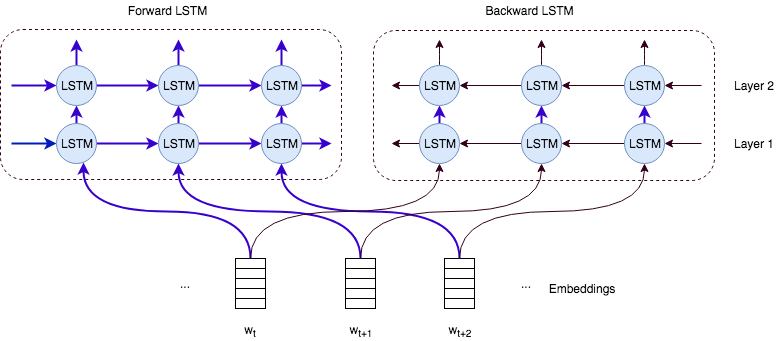
\includegraphics{img/bilstm.png}

Fig 1: 2-layer Bidirectionl LSTM Language Model Architecture

The START and STOP symbols have been added to the sentences in the
generators, and the second dimension of the outputs of generators is the
index of the batch.

\href{https://pytorch.org/tutorials/}{Pytorch} is required in this part.
Do not make any changes to the provided code unless you are requested to
do so.

    \begin{Verbatim}[commandchars=\\\{\}]
{\color{incolor}In [{\color{incolor}5}]:} \PY{c+c1}{\PYZsh{}load packages}
        \PY{k+kn}{import} \PY{n+nn}{torchtext}
        \PY{k+kn}{import} \PY{n+nn}{torch}
        \PY{k+kn}{from} \PY{n+nn}{torchtext}\PY{n+nn}{.}\PY{n+nn}{datasets} \PY{k}{import} \PY{n}{WikiText2}
        \PY{k+kn}{from} \PY{n+nn}{torch} \PY{k}{import} \PY{n}{nn}\PY{p}{,} \PY{n}{optim}
        \PY{k+kn}{from} \PY{n+nn}{torchtext} \PY{k}{import} \PY{n}{data}
        \PY{k+kn}{from} \PY{n+nn}{nltk} \PY{k}{import} \PY{n}{word\PYZus{}tokenize}
        \PY{k+kn}{from} \PY{n+nn}{lstm\PYZus{}model} \PY{k}{import} \PY{n}{LSTMModel}
        \PY{n}{torch}\PY{o}{.}\PY{n}{manual\PYZus{}seed}\PY{p}{(}\PY{l+m+mi}{222}\PY{p}{)}
\end{Verbatim}


\begin{Verbatim}[commandchars=\\\{\}]
{\color{outcolor}Out[{\color{outcolor}5}]:} <torch.\_C.Generator at 0x11aa7a530>
\end{Verbatim}
            
    \begin{Verbatim}[commandchars=\\\{\}]
{\color{incolor}In [{\color{incolor}6}]:} \PY{k}{def} \PY{n+nf}{tokenizer}\PY{p}{(}\PY{n}{text}\PY{p}{)}\PY{p}{:}
            \PY{l+s+sd}{\PYZsq{}\PYZsq{}\PYZsq{}Tokenize a string to words\PYZsq{}\PYZsq{}\PYZsq{}}
            \PY{k}{return} \PY{n}{word\PYZus{}tokenize}\PY{p}{(}\PY{n}{text}\PY{p}{)}
        
        \PY{c+c1}{\PYZsh{}Load and split data into three parts}
        \PY{n}{TEXT} \PY{o}{=} \PY{n}{data}\PY{o}{.}\PY{n}{Field}\PY{p}{(}\PY{n}{lower}\PY{o}{=}\PY{k+kc}{True}\PY{p}{,} \PY{n}{tokenize}\PY{o}{=}\PY{n}{tokenizer}\PY{p}{,} \PY{n}{init\PYZus{}token}\PY{o}{=}\PY{l+s+s1}{\PYZsq{}}\PY{l+s+s1}{\PYZlt{}sos\PYZgt{}}\PY{l+s+s1}{\PYZsq{}}\PY{p}{)}
        \PY{n}{train}\PY{p}{,} \PY{n}{valid}\PY{p}{,} \PY{n}{test} \PY{o}{=} \PY{n}{WikiText2}\PY{o}{.}\PY{n}{splits}\PY{p}{(}\PY{n}{TEXT}\PY{p}{)} 
\end{Verbatim}


    \begin{Verbatim}[commandchars=\\\{\}]
{\color{incolor}In [{\color{incolor}7}]:} \PY{c+c1}{\PYZsh{}Build a vocabulary from the train dataset}
        \PY{n}{TEXT}\PY{o}{.}\PY{n}{build\PYZus{}vocab}\PY{p}{(}\PY{n}{train}\PY{p}{)}
        \PY{n+nb}{print}\PY{p}{(}\PY{l+s+s1}{\PYZsq{}}\PY{l+s+s1}{Vocabulary size:}\PY{l+s+s1}{\PYZsq{}}\PY{p}{,} \PY{n+nb}{len}\PY{p}{(}\PY{n}{TEXT}\PY{o}{.}\PY{n}{vocab}\PY{p}{)}\PY{p}{)}
\end{Verbatim}


    \begin{Verbatim}[commandchars=\\\{\}]
Vocabulary size: 28908

    \end{Verbatim}

    \begin{Verbatim}[commandchars=\\\{\}]
{\color{incolor}In [{\color{incolor}8}]:} \PY{c+c1}{\PYZsh{}Create data generators}
        \PY{n}{BATCH\PYZus{}SIZE} \PY{o}{=} \PY{l+m+mi}{64}
        \PY{n}{BPTT\PYZus{}LEN} \PY{o}{=} \PY{l+m+mi}{32}\PY{c+c1}{\PYZsh{}the length of a text feeding to the RNN layer}
        \PY{n}{train\PYZus{}iter}\PY{p}{,} \PY{n}{valid\PYZus{}iter}\PY{p}{,} \PY{n}{test\PYZus{}iter} \PY{o}{=} \PY{n}{data}\PY{o}{.}\PY{n}{BPTTIterator}\PY{o}{.}\PY{n}{splits}\PY{p}{(}
            \PY{p}{(}\PY{n}{train}\PY{p}{,} \PY{n}{valid}\PY{p}{,} \PY{n}{test}\PY{p}{)}\PY{p}{,}
            \PY{n}{batch\PYZus{}size}\PY{o}{=}\PY{n}{BATCH\PYZus{}SIZE}\PY{p}{,}
            \PY{n}{bptt\PYZus{}len}\PY{o}{=}\PY{l+m+mi}{32}\PY{p}{,}
            \PY{n}{repeat}\PY{o}{=}\PY{k+kc}{False}\PY{p}{)}
\end{Verbatim}


    \begin{Verbatim}[commandchars=\\\{\}]
{\color{incolor}In [{\color{incolor}9}]:} \PY{n+nb}{print}\PY{p}{(}\PY{n+nb}{len}\PY{p}{(}\PY{n}{train\PYZus{}iter}\PY{p}{)}\PY{p}{)}
        \PY{n+nb}{print}\PY{p}{(}\PY{n+nb}{len}\PY{p}{(}\PY{n}{valid\PYZus{}iter}\PY{p}{)}\PY{p}{)}
        \PY{n+nb}{print}\PY{p}{(}\PY{n+nb}{len}\PY{p}{(}\PY{n}{test\PYZus{}iter}\PY{p}{)}\PY{p}{)}
\end{Verbatim}


    \begin{Verbatim}[commandchars=\\\{\}]
1096
121
138

    \end{Verbatim}

    \begin{Verbatim}[commandchars=\\\{\}]
{\color{incolor}In [{\color{incolor}10}]:} \PY{c+c1}{\PYZsh{}Generate a batch of train data}
         \PY{n}{batch} \PY{o}{=} \PY{n+nb}{next}\PY{p}{(}\PY{n+nb}{iter}\PY{p}{(}\PY{n}{train\PYZus{}iter}\PY{p}{)}\PY{p}{)}
         \PY{n}{text}\PY{p}{,} \PY{n}{target} \PY{o}{=} \PY{n}{batch}\PY{o}{.}\PY{n}{text}\PY{p}{,} \PY{n}{batch}\PY{o}{.}\PY{n}{target}
\end{Verbatim}


    \begin{Verbatim}[commandchars=\\\{\}]
{\color{incolor}In [{\color{incolor}11}]:} \PY{n+nb}{print}\PY{p}{(}\PY{l+s+s1}{\PYZsq{}}\PY{l+s+s1}{Size of text tensor}\PY{l+s+s1}{\PYZsq{}}\PY{p}{,}\PY{n}{text}\PY{o}{.}\PY{n}{size}\PY{p}{(}\PY{p}{)}\PY{p}{)}
         \PY{n+nb}{print}\PY{p}{(}\PY{l+s+s1}{\PYZsq{}}\PY{l+s+s1}{Size of target tensor}\PY{l+s+s1}{\PYZsq{}}\PY{p}{,}\PY{n}{target}\PY{o}{.}\PY{n}{size}\PY{p}{(}\PY{p}{)}\PY{p}{)}
\end{Verbatim}


    \begin{Verbatim}[commandchars=\\\{\}]
Size of text tensor torch.Size([32, 64])
Size of target tensor torch.Size([32, 64])

    \end{Verbatim}

    \begin{Verbatim}[commandchars=\\\{\}]
{\color{incolor}In [{\color{incolor}12}]:} \PY{c+c1}{\PYZsh{}\PYZsh{}Write your code here}
         \PY{n}{classifier} \PY{o}{=} \PY{n}{LSTMModel}\PY{p}{(}\PY{n}{vocab\PYZus{}size}\PY{o}{=}\PY{n+nb}{len}\PY{p}{(}\PY{n}{TEXT}\PY{o}{.}\PY{n}{vocab}\PY{p}{)}\PY{p}{,} \PY{n}{emb\PYZus{}size}\PY{o}{=}\PY{l+m+mi}{64}\PY{p}{,} \PY{n}{hidden\PYZus{}size}\PY{o}{=}\PY{l+m+mi}{64}\PY{p}{,} \PY{n}{num\PYZus{}layer}\PY{o}{=}\PY{l+m+mi}{2}\PY{p}{)}
         \PY{n}{optimizer} \PY{o}{=} \PY{n}{torch}\PY{o}{.}\PY{n}{optim}\PY{o}{.}\PY{n}{Adam}\PY{p}{(}\PY{n}{classifier}\PY{o}{.}\PY{n}{parameters}\PY{p}{(}\PY{p}{)}\PY{p}{,} \PY{n}{lr}\PY{o}{=}\PY{l+m+mf}{0.005}\PY{p}{)}
\end{Verbatim}


    \begin{Verbatim}[commandchars=\\\{\}]
{\color{incolor}In [{\color{incolor}13}]:} \PY{k}{def} \PY{n+nf}{trainRNN}\PY{p}{(}\PY{n}{model}\PY{p}{,} \PY{n}{optimizer}\PY{p}{,} \PY{n}{train\PYZus{}iter}\PY{p}{)}\PY{p}{:}
             \PY{n}{criterion} \PY{o}{=} \PY{n}{torch}\PY{o}{.}\PY{n}{nn}\PY{o}{.}\PY{n}{NLLLoss}\PY{p}{(}\PY{p}{)}
             \PY{n}{model}\PY{o}{.}\PY{n}{train}\PY{p}{(}\PY{p}{)}
             \PY{n}{opt\PYZus{}loss} \PY{o}{=} \PY{l+m+mi}{0}
             \PY{n}{hidden} \PY{o}{=} \PY{n}{model}\PY{o}{.}\PY{n}{init\PYZus{}hidden}\PY{p}{(}\PY{l+m+mi}{64}\PY{p}{)}
             \PY{k}{for} \PY{n}{i}\PY{p}{,} \PY{n}{batch} \PY{o+ow}{in} \PY{n+nb}{enumerate}\PY{p}{(}\PY{n}{train\PYZus{}iter}\PY{p}{)}\PY{p}{:}
         \PY{c+c1}{\PYZsh{}         print(batch.target.size())}
                 \PY{n}{optimizer}\PY{o}{.}\PY{n}{zero\PYZus{}grad}\PY{p}{(}\PY{p}{)}
                 \PY{n}{output}\PY{p}{,} \PY{n}{hidden} \PY{o}{=} \PY{n}{model}\PY{p}{(}\PY{n}{batch}\PY{o}{.}\PY{n}{text}\PY{p}{,} \PY{n}{hidden}\PY{p}{)}
         \PY{c+c1}{\PYZsh{}         print(output.size())}
                 \PY{n}{loss} \PY{o}{=} \PY{n}{criterion}\PY{p}{(}\PY{n}{output}\PY{o}{.}\PY{n}{reshape}\PY{p}{(}\PY{p}{[}\PY{l+m+mi}{32}\PY{o}{*}\PY{l+m+mi}{64}\PY{p}{,} \PY{l+m+mi}{28908}\PY{p}{]}\PY{p}{)}\PY{p}{,} \PY{n}{batch}\PY{o}{.}\PY{n}{target}\PY{o}{.}\PY{n}{reshape}\PY{p}{(}\PY{l+m+mi}{32}\PY{o}{*}\PY{l+m+mi}{64}\PY{p}{,}\PY{p}{)}\PY{p}{)}
                 \PY{n}{loss}\PY{o}{.}\PY{n}{backward}\PY{p}{(}\PY{p}{)}
                 \PY{n}{optimizer}\PY{o}{.}\PY{n}{step}\PY{p}{(}\PY{p}{)}
                 \PY{n}{opt\PYZus{}loss} \PY{o}{+}\PY{o}{=} \PY{n}{loss}\PY{o}{.}\PY{n}{item}\PY{p}{(}\PY{p}{)}
                 \PY{k}{if} \PY{n}{i}\PY{o}{\PYZpc{}}\PY{k}{10} == 0 and i != 0:
                     \PY{n+nb}{print}\PY{p}{(}\PY{l+s+s1}{\PYZsq{}}\PY{l+s+s1}{\PYZhy{}\PYZhy{} batch}\PY{l+s+s1}{\PYZsq{}}\PY{p}{,} \PY{n}{i}\PY{p}{,} \PY{l+s+s1}{\PYZsq{}}\PY{l+s+s1}{\PYZhy{}\PYZhy{}}\PY{l+s+s1}{\PYZsq{}}\PY{p}{)}
         \PY{c+c1}{\PYZsh{}             print(torch.argmax(output, 1))}
                     \PY{n+nb}{print}\PY{p}{(}\PY{l+s+s1}{\PYZsq{}}\PY{l+s+s1}{loss}\PY{l+s+s1}{\PYZsq{}}\PY{p}{,} \PY{n}{opt\PYZus{}loss}\PY{o}{/}\PY{n}{i}\PY{p}{)}
             \PY{n+nb}{print}\PY{p}{(}\PY{l+s+s1}{\PYZsq{}}\PY{l+s+s1}{Final training loss is}\PY{l+s+s1}{\PYZsq{}}\PY{p}{,} \PY{n}{opt\PYZus{}loss}\PY{o}{/}\PY{n+nb}{len}\PY{p}{(}\PY{n}{train\PYZus{}iter}\PY{p}{)}\PY{p}{)}
             \PY{k}{return} \PY{n}{opt\PYZus{}loss}\PY{o}{/}\PY{n+nb}{len}\PY{p}{(}\PY{n}{train\PYZus{}iter}\PY{p}{)}
\end{Verbatim}


    \begin{Verbatim}[commandchars=\\\{\}]
{\color{incolor}In [{\color{incolor}14}]:} \PY{n}{opt\PYZus{}loss} \PY{o}{=} \PY{n}{trainRNN}\PY{p}{(}\PY{n}{classifier}\PY{p}{,} \PY{n}{optimizer}\PY{p}{,} \PY{n}{train\PYZus{}iter}\PY{p}{)}
\end{Verbatim}


    \begin{Verbatim}[commandchars=\\\{\}]
-- batch 10 --
loss 10.258363199234008
-- batch 20 --
loss 8.736065244674682
-- batch 30 --
loss 8.237352784474691
-- batch 40 --
loss 7.975195324420929
-- batch 50 --
loss 7.790173187255859
-- batch 60 --
loss 7.659997431437175
-- batch 70 --
loss 7.569610350472587
-- batch 80 --
loss 7.494050419330597
-- batch 90 --
loss 7.437911574045817
-- batch 100 --
loss 7.397030458450318
-- batch 110 --
loss 7.36586233919317
-- batch 120 --
loss 7.330533599853515
-- batch 130 --
loss 7.30030458523677
-- batch 140 --
loss 7.2744867256709504
-- batch 150 --
loss 7.255797344843547
-- batch 160 --
loss 7.236056315898895
-- batch 170 --
loss 7.217669296264648
-- batch 180 --
loss 7.204218623373244
-- batch 190 --
loss 7.1924976800617415
-- batch 200 --
loss 7.182668025493622
-- batch 210 --
loss 7.173686352230254
-- batch 220 --
loss 7.167193235050548
-- batch 230 --
loss 7.158860766369363
-- batch 240 --
loss 7.152265139420828
-- batch 250 --
loss 7.145975580215454
-- batch 260 --
loss 7.140041679602403
-- batch 270 --
loss 7.134516445795695
-- batch 280 --
loss 7.128667085511344
-- batch 290 --
loss 7.12155169125261
-- batch 300 --
loss 7.11583924929301
-- batch 310 --
loss 7.110405888095979
-- batch 320 --
loss 7.104758931696415
-- batch 330 --
loss 7.101091514934193
-- batch 340 --
loss 7.096775273715749
-- batch 350 --
loss 7.0937358638218475
-- batch 360 --
loss 7.090767718685997
-- batch 370 --
loss 7.086581258516054
-- batch 380 --
loss 7.083266436426263
-- batch 390 --
loss 7.077498806439913
-- batch 400 --
loss 7.070760401487351
-- batch 410 --
loss 7.061515455711179
-- batch 420 --
loss 7.053066767965045
-- batch 430 --
loss 7.044179835430412
-- batch 440 --
loss 7.035472019152208
-- batch 450 --
loss 7.026101172765096
-- batch 460 --
loss 7.017540149066759
-- batch 470 --
loss 7.008552099796051
-- batch 480 --
loss 6.997811824083328
-- batch 490 --
loss 6.987714197197739
-- batch 500 --
loss 6.976677969932556
-- batch 510 --
loss 6.96510970732745
-- batch 520 --
loss 6.9547140048100395
-- batch 530 --
loss 6.943819718090993
-- batch 540 --
loss 6.933249402929236
-- batch 550 --
loss 6.922993889721957
-- batch 560 --
loss 6.911683866807393
-- batch 570 --
loss 6.901854173760665
-- batch 580 --
loss 6.891034081886555
-- batch 590 --
loss 6.881904100159467
-- batch 600 --
loss 6.871579299767812
-- batch 610 --
loss 6.861702183426404
-- batch 620 --
loss 6.851953154225503
-- batch 630 --
loss 6.842659077568659
-- batch 640 --
loss 6.8329923816025255
-- batch 650 --
loss 6.823964185714722
-- batch 660 --
loss 6.814899599913395
-- batch 670 --
loss 6.807014915124694
-- batch 680 --
loss 6.799363761088427
-- batch 690 --
loss 6.79148634136587
-- batch 700 --
loss 6.78349682876042
-- batch 710 --
loss 6.7768968985114295
-- batch 720 --
loss 6.769909124904209
-- batch 730 --
loss 6.763804990951329
-- batch 740 --
loss 6.757465396056304
-- batch 750 --
loss 6.7514448172251385
-- batch 760 --
loss 6.744139034497111
-- batch 770 --
loss 6.737702554232114
-- batch 780 --
loss 6.7312764504016975
-- batch 790 --
loss 6.724827822552451
-- batch 800 --
loss 6.718316046595573
-- batch 810 --
loss 6.711869034355069
-- batch 820 --
loss 6.705275516393708
-- batch 830 --
loss 6.698992462617805
-- batch 840 --
loss 6.693119180770148
-- batch 850 --
loss 6.687004141527064
-- batch 860 --
loss 6.681354194463686
-- batch 870 --
loss 6.67529709476164
-- batch 880 --
loss 6.669025299765847
-- batch 890 --
loss 6.6632117833984035
-- batch 900 --
loss 6.6571620315975615
-- batch 910 --
loss 6.652332720389733
-- batch 920 --
loss 6.646847056824228
-- batch 930 --
loss 6.641865942042361
-- batch 940 --
loss 6.637335745831753
-- batch 950 --
loss 6.631898419229608
-- batch 960 --
loss 6.626726633807023
-- batch 970 --
loss 6.621771692983883
-- batch 980 --
loss 6.616724405483324
-- batch 990 --
loss 6.611991964687
-- batch 1000 --
loss 6.6068532056808476
-- batch 1010 --
loss 6.6021004478530125
-- batch 1020 --
loss 6.5976785958981985
-- batch 1030 --
loss 6.593503042332177
-- batch 1040 --
loss 6.588832572331795
-- batch 1050 --
loss 6.58432916368757
-- batch 1060 --
loss 6.579943586295506
-- batch 1070 --
loss 6.574770235792498
-- batch 1080 --
loss 6.569865684156064
-- batch 1090 --
loss 6.5653292546578506
Final training loss is 6.557334312992374

    \end{Verbatim}

    \begin{Verbatim}[commandchars=\\\{\}]
{\color{incolor}In [{\color{incolor}145}]:} \PY{k}{def} \PY{n+nf}{valRNN}\PY{p}{(}\PY{n}{model}\PY{p}{,} \PY{n}{optimizer}\PY{p}{,} \PY{n}{valid\PYZus{}iter}\PY{p}{)}\PY{p}{:}
              \PY{n}{criterion} \PY{o}{=} \PY{n}{torch}\PY{o}{.}\PY{n}{nn}\PY{o}{.}\PY{n}{NLLLoss}\PY{p}{(}\PY{p}{)}
              \PY{n}{model}\PY{o}{.}\PY{n}{eval}\PY{p}{(}\PY{p}{)}
              \PY{n}{opt\PYZus{}loss} \PY{o}{=} \PY{l+m+mi}{0}
              \PY{n}{perplexity} \PY{o}{=} \PY{l+m+mi}{0}
              \PY{n}{hidden} \PY{o}{=} \PY{n}{model}\PY{o}{.}\PY{n}{init\PYZus{}hidden}\PY{p}{(}\PY{l+m+mi}{64}\PY{p}{)}
              \PY{k}{with} \PY{n}{torch}\PY{o}{.}\PY{n}{no\PYZus{}grad}\PY{p}{(}\PY{p}{)}\PY{p}{:}
                  \PY{k}{for} \PY{n}{i}\PY{p}{,} \PY{n}{batch} \PY{o+ow}{in} \PY{n+nb}{enumerate}\PY{p}{(}\PY{n}{valid\PYZus{}iter}\PY{p}{)}\PY{p}{:}
                      \PY{n}{output}\PY{p}{,} \PY{n}{hidden} \PY{o}{=} \PY{n}{model}\PY{p}{(}\PY{n}{batch}\PY{o}{.}\PY{n}{text}\PY{p}{,} \PY{n}{hidden}\PY{p}{)}
                      \PY{n}{loss} \PY{o}{=} \PY{n}{criterion}\PY{p}{(}\PY{n}{output}\PY{o}{.}\PY{n}{reshape}\PY{p}{(}\PY{p}{[}\PY{n}{batch}\PY{o}{.}\PY{n}{text}\PY{o}{.}\PY{n}{size}\PY{p}{(}\PY{p}{)}\PY{p}{[}\PY{l+m+mi}{0}\PY{p}{]}\PY{o}{*}\PY{n}{batch}\PY{o}{.}\PY{n}{text}\PY{o}{.}\PY{n}{size}\PY{p}{(}\PY{p}{)}\PY{p}{[}\PY{l+m+mi}{1}\PY{p}{]}\PY{p}{,} \PY{l+m+mi}{28908}\PY{p}{]}\PY{p}{)}\PY{p}{,} \PY{n}{batch}\PY{o}{.}\PY{n}{target}\PY{o}{.}\PY{n}{reshape}\PY{p}{(}\PY{n}{batch}\PY{o}{.}\PY{n}{text}\PY{o}{.}\PY{n}{size}\PY{p}{(}\PY{p}{)}\PY{p}{[}\PY{l+m+mi}{0}\PY{p}{]}\PY{o}{*}\PY{n}{batch}\PY{o}{.}\PY{n}{text}\PY{o}{.}\PY{n}{size}\PY{p}{(}\PY{p}{)}\PY{p}{[}\PY{l+m+mi}{1}\PY{p}{]}\PY{p}{,}\PY{p}{)}\PY{p}{)}
                      \PY{n}{opt\PYZus{}loss} \PY{o}{+}\PY{o}{=} \PY{n}{loss}\PY{o}{.}\PY{n}{item}\PY{p}{(}\PY{p}{)}
                      
                      \PY{k}{for} \PY{n}{j} \PY{o+ow}{in} \PY{n+nb}{range}\PY{p}{(}\PY{n}{batch}\PY{o}{.}\PY{n}{text}\PY{o}{.}\PY{n}{size}\PY{p}{(}\PY{p}{)}\PY{p}{[}\PY{l+m+mi}{0}\PY{p}{]}\PY{o}{*}\PY{n}{batch}\PY{o}{.}\PY{n}{text}\PY{o}{.}\PY{n}{size}\PY{p}{(}\PY{p}{)}\PY{p}{[}\PY{l+m+mi}{1}\PY{p}{]} \PY{o}{\PYZhy{}} \PY{l+m+mi}{1}\PY{p}{)}\PY{p}{:}
                          \PY{n}{opt\PYZus{}reshape} \PY{o}{=} \PY{n}{output}\PY{o}{.}\PY{n}{reshape}\PY{p}{(}\PY{p}{[}\PY{n}{batch}\PY{o}{.}\PY{n}{text}\PY{o}{.}\PY{n}{size}\PY{p}{(}\PY{p}{)}\PY{p}{[}\PY{l+m+mi}{0}\PY{p}{]}\PY{o}{*}\PY{n}{batch}\PY{o}{.}\PY{n}{text}\PY{o}{.}\PY{n}{size}\PY{p}{(}\PY{p}{)}\PY{p}{[}\PY{l+m+mi}{1}\PY{p}{]}\PY{p}{,} \PY{l+m+mi}{28908}\PY{p}{]}\PY{p}{)}
                          \PY{n}{perplexity} \PY{o}{+}\PY{o}{=} \PY{n}{math}\PY{o}{.}\PY{n}{log2}\PY{p}{(}\PY{n}{math}\PY{o}{.}\PY{n}{exp}\PY{p}{(}\PY{n}{torch}\PY{o}{.}\PY{n}{max}\PY{p}{(}\PY{n}{opt\PYZus{}reshape}\PY{p}{[}\PY{n}{j}\PY{p}{]}\PY{p}{)}\PY{o}{.}\PY{n}{item}\PY{p}{(}\PY{p}{)}\PY{p}{)}\PY{p}{)}
                          
                      \PY{k}{if} \PY{n}{i}\PY{o}{\PYZpc{}}\PY{k}{10} == 0 and i != 0:
                          \PY{n+nb}{print}\PY{p}{(}\PY{l+s+s1}{\PYZsq{}}\PY{l+s+s1}{\PYZhy{}\PYZhy{} batch}\PY{l+s+s1}{\PYZsq{}}\PY{p}{,} \PY{n}{i}\PY{p}{,} \PY{l+s+s1}{\PYZsq{}}\PY{l+s+s1}{\PYZhy{}\PYZhy{}}\PY{l+s+s1}{\PYZsq{}}\PY{p}{)}
                          \PY{n+nb}{print}\PY{p}{(}\PY{l+s+s1}{\PYZsq{}}\PY{l+s+s1}{loss}\PY{l+s+s1}{\PYZsq{}}\PY{p}{,} \PY{n}{opt\PYZus{}loss}\PY{o}{/}\PY{n}{i}\PY{p}{)}
                          \PY{n+nb}{print}\PY{p}{(}\PY{l+s+s1}{\PYZsq{}}\PY{l+s+s1}{perplexity}\PY{l+s+s1}{\PYZsq{}}\PY{p}{,} \PY{n}{math}\PY{o}{.}\PY{n}{pow}\PY{p}{(}\PY{l+m+mi}{2}\PY{p}{,} \PY{o}{\PYZhy{}}\PY{n}{perplexity}\PY{o}{/}\PY{p}{(}\PY{n}{batch}\PY{o}{.}\PY{n}{text}\PY{o}{.}\PY{n}{size}\PY{p}{(}\PY{p}{)}\PY{p}{[}\PY{l+m+mi}{0}\PY{p}{]}\PY{o}{*}\PY{n}{batch}\PY{o}{.}\PY{n}{text}\PY{o}{.}\PY{n}{size}\PY{p}{(}\PY{p}{)}\PY{p}{[}\PY{l+m+mi}{1}\PY{p}{]}\PY{o}{*}\PY{p}{(}\PY{n}{i}\PY{o}{+}\PY{l+m+mi}{1}\PY{p}{)}\PY{p}{)}\PY{p}{)}\PY{p}{)}
              \PY{n+nb}{print}\PY{p}{(}\PY{l+s+s1}{\PYZsq{}}\PY{l+s+s1}{Final testing loss is}\PY{l+s+s1}{\PYZsq{}}\PY{p}{,} \PY{n}{opt\PYZus{}loss}\PY{o}{/}\PY{n+nb}{len}\PY{p}{(}\PY{n}{valid\PYZus{}iter}\PY{p}{)}\PY{p}{)}
              \PY{n+nb}{print}\PY{p}{(}\PY{l+s+s1}{\PYZsq{}}\PY{l+s+s1}{Final perplexity is}\PY{l+s+s1}{\PYZsq{}}\PY{p}{,} \PY{n}{math}\PY{o}{.}\PY{n}{pow}\PY{p}{(}\PY{l+m+mi}{2}\PY{p}{,} \PY{o}{\PYZhy{}}\PY{n}{perplexity}\PY{o}{/}\PY{p}{(}\PY{n}{batch}\PY{o}{.}\PY{n}{text}\PY{o}{.}\PY{n}{size}\PY{p}{(}\PY{p}{)}\PY{p}{[}\PY{l+m+mi}{0}\PY{p}{]}\PY{o}{*}\PY{n}{batch}\PY{o}{.}\PY{n}{text}\PY{o}{.}\PY{n}{size}\PY{p}{(}\PY{p}{)}\PY{p}{[}\PY{l+m+mi}{1}\PY{p}{]}\PY{o}{*}\PY{n+nb}{len}\PY{p}{(}\PY{n}{valid\PYZus{}iter}\PY{p}{)}\PY{p}{)}\PY{p}{)}\PY{p}{)}
              \PY{k}{return} \PY{n}{opt\PYZus{}loss}\PY{o}{/}\PY{n+nb}{len}\PY{p}{(}\PY{n}{valid\PYZus{}iter}\PY{p}{)}\PY{p}{,} \PY{n}{math}\PY{o}{.}\PY{n}{pow}\PY{p}{(}\PY{l+m+mi}{2}\PY{p}{,} \PY{o}{\PYZhy{}}\PY{n}{perplexity}\PY{o}{/}\PY{p}{(}\PY{n}{batch}\PY{o}{.}\PY{n}{text}\PY{o}{.}\PY{n}{size}\PY{p}{(}\PY{p}{)}\PY{p}{[}\PY{l+m+mi}{0}\PY{p}{]}\PY{o}{*}\PY{n}{batch}\PY{o}{.}\PY{n}{text}\PY{o}{.}\PY{n}{size}\PY{p}{(}\PY{p}{)}\PY{p}{[}\PY{l+m+mi}{1}\PY{p}{]}\PY{o}{*}\PY{n+nb}{len}\PY{p}{(}\PY{n}{valid\PYZus{}iter}\PY{p}{)}\PY{p}{)}\PY{p}{)}
\end{Verbatim}


    \begin{Verbatim}[commandchars=\\\{\}]
{\color{incolor}In [{\color{incolor}147}]:} \PY{n}{average\PYZus{}loss}\PY{p}{,} \PY{n}{perplexity} \PY{o}{=} \PY{n}{valRNN}\PY{p}{(}\PY{n}{classifier}\PY{p}{,} \PY{n}{optimizer}\PY{p}{,} \PY{n}{test\PYZus{}iter}\PY{p}{)}
\end{Verbatim}


    \begin{Verbatim}[commandchars=\\\{\}]
-- batch 10 --
loss 5.936151170730591
perplexity 9.334124180994229
-- batch 20 --
loss 5.637724566459656
perplexity 9.199409903166883
-- batch 30 --
loss 5.526246436436971
perplexity 9.136797046079236
-- batch 40 --
loss 5.450850188732147
perplexity 9.04350470698952
-- batch 50 --
loss 5.428130693435669
perplexity 9.032847883100086
-- batch 60 --
loss 5.418380069732666
perplexity 9.03729440707681
-- batch 70 --
loss 5.408901493889945
perplexity 9.04267573164418
-- batch 80 --
loss 5.392224472761154
perplexity 9.017739650174088
-- batch 90 --
loss 5.390909915500217
perplexity 9.045350797624058
-- batch 100 --
loss 5.378343224525452
perplexity 9.038449614109773
-- batch 110 --
loss 5.374320680444891
perplexity 9.042114526538324
-- batch 120 --
loss 5.370130678017934
perplexity 9.045233756370951
-- batch 130 --
loss 5.365696305495042
perplexity 9.041088841185747
Final testing loss is 5.326513908911442
Final perplexity is 16.693741082730547

    \end{Verbatim}

    \begin{Verbatim}[commandchars=\\\{\}]
{\color{incolor}In [{\color{incolor}15}]:} \PY{c+c1}{\PYZsh{}\PYZsh{}\PYZsh{} Visualize}
         \PY{k+kn}{import} \PY{n+nn}{numpy} \PY{k}{as} \PY{n+nn}{np}
         \PY{n}{embbeding} \PY{o}{=} \PY{n}{classifier}\PY{o}{.}\PY{n}{encoder}
\end{Verbatim}


    \begin{Verbatim}[commandchars=\\\{\}]
{\color{incolor}In [{\color{incolor}16}]:} \PY{k}{def} \PY{n+nf}{PCA}\PY{p}{(}\PY{n}{X}\PY{p}{,} \PY{n}{k}\PY{o}{=}\PY{l+m+mi}{2}\PY{p}{)}\PY{p}{:}
          \PY{c+c1}{\PYZsh{} preprocess the data}
          \PY{n}{X\PYZus{}mean} \PY{o}{=} \PY{n}{torch}\PY{o}{.}\PY{n}{mean}\PY{p}{(}\PY{n}{X}\PY{p}{,}\PY{l+m+mi}{0}\PY{p}{)}
          \PY{n}{X} \PY{o}{=} \PY{n}{X} \PY{o}{\PYZhy{}} \PY{n}{X\PYZus{}mean}\PY{o}{.}\PY{n}{expand\PYZus{}as}\PY{p}{(}\PY{n}{X}\PY{p}{)}
         
          \PY{c+c1}{\PYZsh{} svd}
          \PY{n}{U}\PY{p}{,}\PY{n}{S}\PY{p}{,}\PY{n}{V} \PY{o}{=} \PY{n}{torch}\PY{o}{.}\PY{n}{svd}\PY{p}{(}\PY{n}{torch}\PY{o}{.}\PY{n}{t}\PY{p}{(}\PY{n}{X}\PY{p}{)}\PY{p}{)}
          \PY{k}{return} \PY{n}{torch}\PY{o}{.}\PY{n}{mm}\PY{p}{(}\PY{n}{X}\PY{p}{,}\PY{n}{U}\PY{p}{[}\PY{p}{:}\PY{p}{,}\PY{p}{:}\PY{n}{k}\PY{p}{]}\PY{p}{)}
\end{Verbatim}


    \begin{Verbatim}[commandchars=\\\{\}]
{\color{incolor}In [{\color{incolor}17}]:} \PY{n}{embedding\PYZus{}pca} \PY{o}{=} \PY{n}{PCA}\PY{p}{(}\PY{n}{embbeding}\PY{o}{.}\PY{n}{weight}\PY{p}{)}
\end{Verbatim}


    \begin{Verbatim}[commandchars=\\\{\}]
{\color{incolor}In [{\color{incolor}18}]:} \PY{k+kn}{import} \PY{n+nn}{matplotlib}\PY{n+nn}{.}\PY{n+nn}{pyplot} \PY{k}{as} \PY{n+nn}{plt}
         \PY{k}{def} \PY{n+nf}{plot}\PY{p}{(}\PY{n}{embeddings}\PY{p}{,} \PY{n}{labels}\PY{p}{)}\PY{p}{:}
           \PY{k}{assert} \PY{n}{embeddings}\PY{o}{.}\PY{n}{shape}\PY{p}{[}\PY{l+m+mi}{0}\PY{p}{]} \PY{o}{\PYZgt{}}\PY{o}{=} \PY{n+nb}{len}\PY{p}{(}\PY{n}{labels}\PY{p}{)}\PY{p}{,} \PY{l+s+s1}{\PYZsq{}}\PY{l+s+s1}{More labels than embeddings}\PY{l+s+s1}{\PYZsq{}}
           \PY{n}{plt}\PY{o}{.}\PY{n}{figure}\PY{p}{(}\PY{n}{figsize}\PY{o}{=}\PY{p}{(}\PY{l+m+mi}{15}\PY{p}{,}\PY{l+m+mi}{15}\PY{p}{)}\PY{p}{)}  \PY{c+c1}{\PYZsh{} in inches}
           \PY{k}{for} \PY{n}{i}\PY{p}{,} \PY{n}{label} \PY{o+ow}{in} \PY{n+nb}{enumerate}\PY{p}{(}\PY{n}{labels}\PY{p}{)}\PY{p}{:}
             \PY{n}{x}\PY{p}{,} \PY{n}{y} \PY{o}{=} \PY{n}{embeddings}\PY{p}{[}\PY{n}{i}\PY{p}{,}\PY{p}{:}\PY{p}{]}
             \PY{n}{plt}\PY{o}{.}\PY{n}{scatter}\PY{p}{(}\PY{n}{x}\PY{p}{,} \PY{n}{y}\PY{p}{)}
             \PY{n}{plt}\PY{o}{.}\PY{n}{annotate}\PY{p}{(}\PY{n}{label}\PY{p}{,} \PY{n}{xy}\PY{o}{=}\PY{p}{(}\PY{n}{x}\PY{p}{,} \PY{n}{y}\PY{p}{)}\PY{p}{,} \PY{n}{xytext}\PY{o}{=}\PY{p}{(}\PY{l+m+mi}{5}\PY{p}{,} \PY{l+m+mi}{2}\PY{p}{)}\PY{p}{,} \PY{n}{textcoords}\PY{o}{=}\PY{l+s+s1}{\PYZsq{}}\PY{l+s+s1}{offset points}\PY{l+s+s1}{\PYZsq{}}\PY{p}{,}
                            \PY{n}{ha}\PY{o}{=}\PY{l+s+s1}{\PYZsq{}}\PY{l+s+s1}{right}\PY{l+s+s1}{\PYZsq{}}\PY{p}{,} \PY{n}{va}\PY{o}{=}\PY{l+s+s1}{\PYZsq{}}\PY{l+s+s1}{bottom}\PY{l+s+s1}{\PYZsq{}}\PY{p}{)}
\end{Verbatim}


    \begin{Verbatim}[commandchars=\\\{\}]
{\color{incolor}In [{\color{incolor}26}]:} \PY{n}{plot}\PY{p}{(}\PY{n}{embedding\PYZus{}pca}\PY{o}{.}\PY{n}{detach}\PY{p}{(}\PY{p}{)}\PY{o}{.}\PY{n}{numpy}\PY{p}{(}\PY{p}{)}\PY{p}{[}\PY{l+m+mi}{1}\PY{p}{:}\PY{l+m+mi}{300}\PY{p}{,} \PY{p}{:}\PY{p}{]}\PY{p}{,} \PY{n}{TEXT}\PY{o}{.}\PY{n}{vocab}\PY{o}{.}\PY{n}{itos}\PY{p}{[}\PY{l+m+mi}{1}\PY{p}{:}\PY{l+m+mi}{300}\PY{p}{]}\PY{p}{)}
\end{Verbatim}


    \begin{center}
    \adjustimage{max size={0.9\linewidth}{0.9\paperheight}}{output_45_0.png}
    \end{center}
    { \hspace*{\fill} \\}
    
    \begin{Verbatim}[commandchars=\\\{\}]
{\color{incolor}In [{\color{incolor}13}]:} \PY{c+c1}{\PYZsh{}\PYZsh{}\PYZsh{} Bi directional LSTM}
         \PY{k}{class} \PY{n+nc}{BILSTMModel}\PY{p}{(}\PY{n}{LSTMModel}\PY{p}{)}\PY{p}{:}
             \PY{k}{def} \PY{n+nf}{\PYZus{}\PYZus{}init\PYZus{}\PYZus{}}\PY{p}{(}\PY{n+nb+bp}{self}\PY{p}{,} \PY{n}{vocab\PYZus{}size}\PY{p}{,} \PY{n}{emb\PYZus{}size}\PY{p}{,} \PY{n}{hidden\PYZus{}size}\PY{p}{,} \PY{n}{num\PYZus{}layer}\PY{p}{,} \PY{n}{dropout}\PY{o}{=}\PY{l+m+mf}{0.5}\PY{p}{)}\PY{p}{:}
                 \PY{n+nb}{super}\PY{p}{(}\PY{n}{LSTMModel}\PY{p}{,} \PY{n+nb+bp}{self}\PY{p}{)}\PY{o}{.}\PY{n+nf+fm}{\PYZus{}\PYZus{}init\PYZus{}\PYZus{}}\PY{p}{(}\PY{p}{)}
                 \PY{n+nb+bp}{self}\PY{o}{.}\PY{n}{hidden\PYZus{}size}\PY{p}{,} \PY{n+nb+bp}{self}\PY{o}{.}\PY{n}{num\PYZus{}layer} \PY{o}{=} \PY{n}{hidden\PYZus{}size}\PY{p}{,} \PY{n}{num\PYZus{}layer}
                 \PY{n+nb+bp}{self}\PY{o}{.}\PY{n}{drop} \PY{o}{=} \PY{n}{nn}\PY{o}{.}\PY{n}{Dropout}\PY{p}{(}\PY{n}{dropout}\PY{p}{)}
                 \PY{n+nb+bp}{self}\PY{o}{.}\PY{n}{encoder} \PY{o}{=} \PY{n}{nn}\PY{o}{.}\PY{n}{Embedding}\PY{p}{(}\PY{n}{vocab\PYZus{}size}\PY{p}{,} \PY{n}{emb\PYZus{}size}\PY{p}{)}
                 \PY{n+nb+bp}{self}\PY{o}{.}\PY{n}{frnn} \PY{o}{=} \PY{n}{nn}\PY{o}{.}\PY{n}{LSTM}\PY{p}{(}\PY{n}{emb\PYZus{}size}\PY{p}{,} \PY{n}{hidden\PYZus{}size}\PY{p}{,} \PY{n}{num\PYZus{}layer}\PY{p}{,} \PY{n}{dropout}\PY{o}{=}\PY{n}{dropout}\PY{p}{)}
                 \PY{n+nb+bp}{self}\PY{o}{.}\PY{n}{brnn} \PY{o}{=} \PY{n}{nn}\PY{o}{.}\PY{n}{LSTM}\PY{p}{(}\PY{n}{emb\PYZus{}size}\PY{p}{,} \PY{n}{hidden\PYZus{}size}\PY{p}{,} \PY{n}{num\PYZus{}layer}\PY{p}{,} \PY{n}{dropout}\PY{o}{=}\PY{n}{dropout}\PY{p}{)}
                 \PY{n+nb+bp}{self}\PY{o}{.}\PY{n}{decoder} \PY{o}{=} \PY{n}{nn}\PY{o}{.}\PY{n}{Linear}\PY{p}{(}\PY{n}{hidden\PYZus{}size}\PY{p}{,} \PY{n}{vocab\PYZus{}size}\PY{p}{)}
                 \PY{n+nb+bp}{self}\PY{o}{.}\PY{n}{softmax} \PY{o}{=} \PY{n}{nn}\PY{o}{.}\PY{n}{Softmax}\PY{p}{(}\PY{n}{dim}\PY{o}{=}\PY{l+m+mi}{2}\PY{p}{)}
                 \PY{n+nb+bp}{self}\PY{o}{.}\PY{n}{init\PYZus{}weights}\PY{p}{(}\PY{p}{)}
                 
             \PY{k}{def} \PY{n+nf}{forward}\PY{p}{(}\PY{n+nb+bp}{self}\PY{p}{,} \PY{n}{input\PYZus{}tensor}\PY{p}{,} \PY{n}{fhidden}\PY{p}{,} \PY{n}{bhidden}\PY{p}{)}\PY{p}{:}
                 \PY{c+c1}{\PYZsh{}Get embeddings for the input tensors}
                 \PY{n}{emb} \PY{o}{=} \PY{n+nb+bp}{self}\PY{o}{.}\PY{n}{encoder}\PY{p}{(}\PY{n}{input\PYZus{}tensor}\PY{p}{)}
                 \PY{c+c1}{\PYZsh{}dropout}
                 \PY{n}{emb} \PY{o}{=} \PY{n+nb+bp}{self}\PY{o}{.}\PY{n}{drop}\PY{p}{(}\PY{n}{emb}\PY{p}{)}
                 \PY{c+c1}{\PYZsh{}Remove history of hidden states}
                 \PY{n}{fhidden} \PY{o}{=} \PY{n+nb+bp}{self}\PY{o}{.}\PY{n}{repackage\PYZus{}hidden}\PY{p}{(}\PY{n}{fhidden}\PY{p}{)}
                 \PY{n}{bhidden} \PY{o}{=} \PY{n+nb+bp}{self}\PY{o}{.}\PY{n}{repackage\PYZus{}hidden}\PY{p}{(}\PY{n}{bhidden}\PY{p}{)}
                 \PY{c+c1}{\PYZsh{}rnn layer}
         \PY{c+c1}{\PYZsh{}         print(emb.size())}
                 \PY{n}{foutput}\PY{p}{,} \PY{n}{fhidden} \PY{o}{=} \PY{n+nb+bp}{self}\PY{o}{.}\PY{n}{frnn}\PY{p}{(}\PY{n}{emb}\PY{p}{,} \PY{n}{fhidden}\PY{p}{)}
                 \PY{n}{boutput}\PY{p}{,} \PY{n}{bhidden} \PY{o}{=} \PY{n+nb+bp}{self}\PY{o}{.}\PY{n}{brnn}\PY{p}{(}\PY{n}{torch}\PY{o}{.}\PY{n}{flip}\PY{p}{(}\PY{n}{emb}\PY{p}{,} \PY{p}{[}\PY{l+m+mi}{0}\PY{p}{,} \PY{l+m+mi}{1}\PY{p}{]}\PY{p}{)}\PY{p}{,} \PY{n}{bhidden}\PY{p}{)}
                 \PY{c+c1}{\PYZsh{}dropout}
                 \PY{n}{foutput} \PY{o}{=} \PY{n+nb+bp}{self}\PY{o}{.}\PY{n}{drop}\PY{p}{(}\PY{n}{foutput}\PY{p}{)}
                 \PY{n}{boutput} \PY{o}{=} \PY{n+nb+bp}{self}\PY{o}{.}\PY{n}{drop}\PY{p}{(}\PY{n}{boutput}\PY{p}{)}
                 \PY{n}{fdecoded} \PY{o}{=} \PY{n+nb+bp}{self}\PY{o}{.}\PY{n}{decoder}\PY{p}{(}\PY{n}{foutput}\PY{o}{.}\PY{n}{view}\PY{p}{(}\PY{n}{foutput}\PY{o}{.}\PY{n}{size}\PY{p}{(}\PY{l+m+mi}{0}\PY{p}{)}\PY{o}{*}\PY{n}{foutput}\PY{o}{.}\PY{n}{size}\PY{p}{(}\PY{l+m+mi}{1}\PY{p}{)}\PY{p}{,} \PY{n}{foutput}\PY{o}{.}\PY{n}{size}\PY{p}{(}\PY{l+m+mi}{2}\PY{p}{)}\PY{p}{)}\PY{p}{)}
                 \PY{n}{bdecoded} \PY{o}{=} \PY{n+nb+bp}{self}\PY{o}{.}\PY{n}{decoder}\PY{p}{(}\PY{n}{boutput}\PY{o}{.}\PY{n}{view}\PY{p}{(}\PY{n}{boutput}\PY{o}{.}\PY{n}{size}\PY{p}{(}\PY{l+m+mi}{0}\PY{p}{)}\PY{o}{*}\PY{n}{boutput}\PY{o}{.}\PY{n}{size}\PY{p}{(}\PY{l+m+mi}{1}\PY{p}{)}\PY{p}{,} \PY{n}{boutput}\PY{o}{.}\PY{n}{size}\PY{p}{(}\PY{l+m+mi}{2}\PY{p}{)}\PY{p}{)}\PY{p}{)}
                 \PY{n}{foutputs} \PY{o}{=} \PY{n}{fdecoded}\PY{o}{.}\PY{n}{view}\PY{p}{(}\PY{n}{foutput}\PY{o}{.}\PY{n}{size}\PY{p}{(}\PY{l+m+mi}{0}\PY{p}{)}\PY{p}{,} \PY{n}{foutput}\PY{o}{.}\PY{n}{size}\PY{p}{(}\PY{l+m+mi}{1}\PY{p}{)}\PY{p}{,} \PY{n}{fdecoded}\PY{o}{.}\PY{n}{size}\PY{p}{(}\PY{l+m+mi}{1}\PY{p}{)}\PY{p}{)}
                 \PY{n}{boutputs} \PY{o}{=} \PY{n}{bdecoded}\PY{o}{.}\PY{n}{view}\PY{p}{(}\PY{n}{boutput}\PY{o}{.}\PY{n}{size}\PY{p}{(}\PY{l+m+mi}{0}\PY{p}{)}\PY{p}{,} \PY{n}{boutput}\PY{o}{.}\PY{n}{size}\PY{p}{(}\PY{l+m+mi}{1}\PY{p}{)}\PY{p}{,} \PY{n}{bdecoded}\PY{o}{.}\PY{n}{size}\PY{p}{(}\PY{l+m+mi}{1}\PY{p}{)}\PY{p}{)}
                 \PY{c+c1}{\PYZsh{}Compute the softmax values}
                 \PY{n}{foutputs} \PY{o}{=} \PY{n+nb+bp}{self}\PY{o}{.}\PY{n}{softmax}\PY{p}{(}\PY{n}{foutputs}\PY{p}{)}
                 \PY{n}{boutputs} \PY{o}{=} \PY{n+nb+bp}{self}\PY{o}{.}\PY{n}{softmax}\PY{p}{(}\PY{n}{boutputs}\PY{p}{)}
                 \PY{c+c1}{\PYZsh{}Set the values within a range}
                 \PY{n}{foutputs} \PY{o}{=} \PY{n}{torch}\PY{o}{.}\PY{n}{clamp}\PY{p}{(}\PY{n}{foutputs}\PY{p}{,} \PY{n+nb}{min}\PY{o}{=}\PY{l+m+mf}{0.000000001}\PY{p}{,} \PY{n+nb}{max}\PY{o}{=}\PY{l+m+mi}{100000}\PY{p}{)}
                 \PY{n}{boutputs} \PY{o}{=} \PY{n}{torch}\PY{o}{.}\PY{n}{clamp}\PY{p}{(}\PY{n}{boutputs}\PY{p}{,} \PY{n+nb}{min}\PY{o}{=}\PY{l+m+mf}{0.000000001}\PY{p}{,} \PY{n+nb}{max}\PY{o}{=}\PY{l+m+mi}{100000}\PY{p}{)}
                 \PY{c+c1}{\PYZsh{}Compute log values}
                 \PY{n}{foutputs} \PY{o}{=} \PY{n}{torch}\PY{o}{.}\PY{n}{log}\PY{p}{(}\PY{n}{foutputs}\PY{p}{)}
                 \PY{n}{boutputs} \PY{o}{=} \PY{n}{torch}\PY{o}{.}\PY{n}{log}\PY{p}{(}\PY{n}{boutputs}\PY{p}{)}
                 \PY{k}{return} \PY{n}{foutputs}\PY{p}{,} \PY{n}{torch}\PY{o}{.}\PY{n}{flip}\PY{p}{(}\PY{n}{boutputs}\PY{p}{,} \PY{p}{[}\PY{l+m+mi}{0}\PY{p}{,} \PY{l+m+mi}{1}\PY{p}{]}\PY{p}{)}\PY{p}{,} \PY{n}{fhidden}\PY{p}{,} \PY{n}{bhidden}
\end{Verbatim}


    \begin{Verbatim}[commandchars=\\\{\}]
{\color{incolor}In [{\color{incolor}14}]:} \PY{n}{bi\PYZus{}classifier} \PY{o}{=} \PY{n}{BILSTMModel}\PY{p}{(}\PY{n}{vocab\PYZus{}size}\PY{o}{=}\PY{n+nb}{len}\PY{p}{(}\PY{n}{TEXT}\PY{o}{.}\PY{n}{vocab}\PY{p}{)}\PY{p}{,} \PY{n}{emb\PYZus{}size}\PY{o}{=}\PY{l+m+mi}{64}\PY{p}{,} \PY{n}{hidden\PYZus{}size}\PY{o}{=}\PY{l+m+mi}{64}\PY{p}{,} \PY{n}{num\PYZus{}layer}\PY{o}{=}\PY{l+m+mi}{2}\PY{p}{)}
         \PY{n}{optimizer} \PY{o}{=} \PY{n}{torch}\PY{o}{.}\PY{n}{optim}\PY{o}{.}\PY{n}{Adam}\PY{p}{(}\PY{n}{classifier}\PY{o}{.}\PY{n}{parameters}\PY{p}{(}\PY{p}{)}\PY{p}{,} \PY{n}{lr}\PY{o}{=}\PY{l+m+mf}{0.005}\PY{p}{)}
\end{Verbatim}


    \begin{Verbatim}[commandchars=\\\{\}]
{\color{incolor}In [{\color{incolor}20}]:} \PY{k}{def} \PY{n+nf}{trainBIRNN}\PY{p}{(}\PY{n}{model}\PY{p}{,} \PY{n}{optimizer}\PY{p}{,} \PY{n}{train\PYZus{}iter}\PY{p}{)}\PY{p}{:}
             \PY{n}{criterion} \PY{o}{=} \PY{n}{torch}\PY{o}{.}\PY{n}{nn}\PY{o}{.}\PY{n}{NLLLoss}\PY{p}{(}\PY{p}{)}
             \PY{n}{model}\PY{o}{.}\PY{n}{train}\PY{p}{(}\PY{p}{)}
             \PY{n}{fopt\PYZus{}loss} \PY{o}{=} \PY{l+m+mi}{0}
             \PY{n}{bopt\PYZus{}loss} \PY{o}{=} \PY{l+m+mi}{0}
             \PY{n}{fhidden} \PY{o}{=} \PY{n}{model}\PY{o}{.}\PY{n}{init\PYZus{}hidden}\PY{p}{(}\PY{l+m+mi}{64}\PY{p}{)}
             \PY{n}{bhidden} \PY{o}{=} \PY{n}{model}\PY{o}{.}\PY{n}{init\PYZus{}hidden}\PY{p}{(}\PY{l+m+mi}{64}\PY{p}{)}
             \PY{k}{for} \PY{n}{i}\PY{p}{,} \PY{n}{batch} \PY{o+ow}{in} \PY{n+nb}{enumerate}\PY{p}{(}\PY{n}{train\PYZus{}iter}\PY{p}{)}\PY{p}{:}
         \PY{c+c1}{\PYZsh{}         print(batch.target.size())}
                 \PY{n}{optimizer}\PY{o}{.}\PY{n}{zero\PYZus{}grad}\PY{p}{(}\PY{p}{)}
                 \PY{n}{foutput}\PY{p}{,} \PY{n}{boutput}\PY{p}{,} \PY{n}{fhidden}\PY{p}{,} \PY{n}{bhidden} \PY{o}{=} \PY{n}{model}\PY{p}{(}\PY{n}{batch}\PY{o}{.}\PY{n}{text}\PY{p}{,} \PY{n}{fhidden}\PY{p}{,} \PY{n}{bhidden}\PY{p}{)}
         \PY{c+c1}{\PYZsh{}         print(output.size())}
                 \PY{n}{floss} \PY{o}{=} \PY{n}{criterion}\PY{p}{(}\PY{n}{foutput}\PY{o}{.}\PY{n}{reshape}\PY{p}{(}\PY{p}{[}\PY{l+m+mi}{32}\PY{o}{*}\PY{l+m+mi}{64}\PY{p}{,} \PY{l+m+mi}{28908}\PY{p}{]}\PY{p}{)}\PY{p}{,} \PY{n}{batch}\PY{o}{.}\PY{n}{target}\PY{o}{.}\PY{n}{reshape}\PY{p}{(}\PY{l+m+mi}{32}\PY{o}{*}\PY{l+m+mi}{64}\PY{p}{,}\PY{p}{)}\PY{p}{)}
                 \PY{n}{bloss} \PY{o}{=} \PY{n}{criterion}\PY{p}{(}\PY{n}{boutput}\PY{o}{.}\PY{n}{reshape}\PY{p}{(}\PY{p}{[}\PY{l+m+mi}{32}\PY{o}{*}\PY{l+m+mi}{64}\PY{p}{,} \PY{l+m+mi}{28908}\PY{p}{]}\PY{p}{)}\PY{p}{,} \PY{n}{batch}\PY{o}{.}\PY{n}{target}\PY{o}{.}\PY{n}{reshape}\PY{p}{(}\PY{l+m+mi}{32}\PY{o}{*}\PY{l+m+mi}{64}\PY{p}{,}\PY{p}{)}\PY{p}{)}
                 \PY{n}{model}\PY{o}{.}\PY{n}{frnn}\PY{o}{.}\PY{n}{requires\PYZus{}grad} \PY{o}{=} \PY{k+kc}{True}
                 \PY{n}{model}\PY{o}{.}\PY{n}{brnn}\PY{o}{.}\PY{n}{requires\PYZus{}grad} \PY{o}{=} \PY{k+kc}{False}
                 \PY{n}{floss}\PY{o}{.}\PY{n}{backward}\PY{p}{(}\PY{n}{retain\PYZus{}graph}\PY{o}{=}\PY{k+kc}{True}\PY{p}{)}
                 \PY{n}{optimizer}\PY{o}{.}\PY{n}{step}\PY{p}{(}\PY{p}{)}
                 
                 \PY{n}{model}\PY{o}{.}\PY{n}{brnn}\PY{o}{.}\PY{n}{requires\PYZus{}grad} \PY{o}{=} \PY{k+kc}{True}
                 \PY{n}{model}\PY{o}{.}\PY{n}{frnn}\PY{o}{.}\PY{n}{requires\PYZus{}grad} \PY{o}{=} \PY{k+kc}{False}
                 \PY{n}{bloss}\PY{o}{.}\PY{n}{backward}\PY{p}{(}\PY{n}{retain\PYZus{}graph}\PY{o}{=}\PY{k+kc}{True}\PY{p}{)}
                 \PY{n}{optimizer}\PY{o}{.}\PY{n}{step}\PY{p}{(}\PY{p}{)}
                 \PY{n}{fopt\PYZus{}loss} \PY{o}{+}\PY{o}{=} \PY{n}{floss}\PY{o}{.}\PY{n}{item}\PY{p}{(}\PY{p}{)}
                 \PY{n}{bopt\PYZus{}loss} \PY{o}{+}\PY{o}{=} \PY{n}{bloss}\PY{o}{.}\PY{n}{item}\PY{p}{(}\PY{p}{)}
                 \PY{k}{if} \PY{n}{i}\PY{o}{\PYZpc{}}\PY{k}{10} == 0 and i != 0:
                     \PY{n+nb}{print}\PY{p}{(}\PY{l+s+s1}{\PYZsq{}}\PY{l+s+s1}{\PYZhy{}\PYZhy{} batch}\PY{l+s+s1}{\PYZsq{}}\PY{p}{,} \PY{n}{i}\PY{p}{,} \PY{l+s+s1}{\PYZsq{}}\PY{l+s+s1}{\PYZhy{}\PYZhy{}}\PY{l+s+s1}{\PYZsq{}}\PY{p}{)}
         \PY{c+c1}{\PYZsh{}             print(torch.argmax(output, 1))}
                     \PY{n+nb}{print}\PY{p}{(}\PY{l+s+s1}{\PYZsq{}}\PY{l+s+s1}{forward loss}\PY{l+s+s1}{\PYZsq{}}\PY{p}{,} \PY{n}{fopt\PYZus{}loss}\PY{o}{/}\PY{n}{i}\PY{p}{)}
                     \PY{n+nb}{print}\PY{p}{(}\PY{l+s+s1}{\PYZsq{}}\PY{l+s+s1}{backward loss}\PY{l+s+s1}{\PYZsq{}}\PY{p}{,} \PY{n}{bopt\PYZus{}loss}\PY{o}{/}\PY{n}{i}\PY{p}{)}
             \PY{n+nb}{print}\PY{p}{(}\PY{l+s+s1}{\PYZsq{}}\PY{l+s+s1}{Final forward training loss is}\PY{l+s+s1}{\PYZsq{}}\PY{p}{,} \PY{n}{fopt\PYZus{}loss}\PY{o}{/}\PY{n+nb}{len}\PY{p}{(}\PY{n}{train\PYZus{}iter}\PY{p}{)}\PY{p}{)}
             \PY{n+nb}{print}\PY{p}{(}\PY{l+s+s1}{\PYZsq{}}\PY{l+s+s1}{Final backward training loss is}\PY{l+s+s1}{\PYZsq{}}\PY{p}{,} \PY{n}{bopt\PYZus{}loss}\PY{o}{/}\PY{n+nb}{len}\PY{p}{(}\PY{n}{train\PYZus{}iter}\PY{p}{)}\PY{p}{)}
             \PY{k}{return} \PY{n}{fopt\PYZus{}loss}\PY{o}{/}\PY{n+nb}{len}\PY{p}{(}\PY{n}{train\PYZus{}iter}\PY{p}{)}\PY{p}{,} \PY{n}{bopt\PYZus{}loss}\PY{o}{/}\PY{n+nb}{len}\PY{p}{(}\PY{n}{train\PYZus{}iter}\PY{p}{)}
\end{Verbatim}


    \begin{Verbatim}[commandchars=\\\{\}]
{\color{incolor}In [{\color{incolor}177}]:} \PY{n}{fopt\PYZus{}loss}\PY{p}{,} \PY{n}{bopt\PYZus{}loss} \PY{o}{=} \PY{n}{trainBIRNN}\PY{p}{(}\PY{n}{bi\PYZus{}classifier}\PY{p}{,} \PY{n}{optimizer}\PY{p}{,} \PY{n}{train\PYZus{}iter}\PY{p}{)}
\end{Verbatim}


    \begin{Verbatim}[commandchars=\\\{\}]
-- batch 10 --
forward loss 11.297070980072021
backward loss 11.29778175354004
-- batch 20 --
forward loss 10.783352422714234
backward loss 10.784309530258179
-- batch 30 --
forward loss 10.612307929992676
backward loss 10.613202540079753
-- batch 40 --
forward loss 10.526631784439086
backward loss 10.527464270591736
-- batch 50 --
forward loss 10.47527006149292
backward loss 10.476182594299317
-- batch 60 --
forward loss 10.440999873479207
backward loss 10.441911315917968
-- batch 70 --
forward loss 10.416552366529192
backward loss 10.417428289140974
-- batch 80 --
forward loss 10.398204267024994
backward loss 10.399112904071808
-- batch 90 --
forward loss 10.38395651711358
backward loss 10.384820493062337
-- batch 100 --
forward loss 10.372553281784057
backward loss 10.373407726287843
-- batch 110 --
forward loss 10.363234329223634
backward loss 10.364042516188189
-- batch 120 --
forward loss 10.355453944206237
backward loss 10.356258138020833
-- batch 130 --
forward loss 10.348850734417255
backward loss 10.349671481205867
-- batch 140 --
forward loss 10.343220220293318
backward loss 10.344035625457764
-- batch 150 --
forward loss 10.338309326171874
backward loss 10.339151446024577
-- batch 160 --
forward loss 10.334004372358322
backward loss 10.334859478473664
-- batch 170 --
forward loss 10.330200498244341
backward loss 10.331068151137409
-- batch 180 --
forward loss 10.326837232377795
backward loss 10.327713600794475
-- batch 190 --
forward loss 10.32382106279072
backward loss 10.324711056759483
-- batch 200 --
forward loss 10.321113209724427
backward loss 10.322013039588928
-- batch 210 --
forward loss 10.318675754183815
backward loss 10.319565981910342
-- batch 220 --
forward loss 10.316472586718472
backward loss 10.317374177412553
-- batch 230 --
forward loss 10.314449198349662
backward loss 10.315337085723877
-- batch 240 --
forward loss 10.312605373064677
backward loss 10.313475255171458
-- batch 250 --
forward loss 10.310893672943115
backward loss 10.311768447875977
-- batch 260 --
forward loss 10.309324895418607
backward loss 10.310203108420739
-- batch 270 --
forward loss 10.307855524840178
backward loss 10.308738351751257
-- batch 280 --
forward loss 10.306528438840594
backward loss 10.307394337654113
-- batch 290 --
forward loss 10.305272546307794
backward loss 10.306124874641155
-- batch 300 --
forward loss 10.304115263621012
backward loss 10.30493237177531
-- batch 310 --
forward loss 10.30302309220837
backward loss 10.3038268919914
-- batch 320 --
forward loss 10.302004224061966
backward loss 10.302806946635247
-- batch 330 --
forward loss 10.301024954246753
backward loss 10.301832334923022
-- batch 340 --
forward loss 10.300091443342321
backward loss 10.300913202061373
-- batch 350 --
forward loss 10.2992215020316
backward loss 10.30005016054426
-- batch 360 --
forward loss 10.298408272531297
backward loss 10.299235894944932
-- batch 370 --
forward loss 10.297633395323881
backward loss 10.298464099780933
-- batch 380 --
forward loss 10.296910436529862
backward loss 10.297736363661917
-- batch 390 --
forward loss 10.296208731333415
backward loss 10.297039753351456
-- batch 400 --
forward loss 10.295549392700195
backward loss 10.296370797157287
-- batch 410 --
forward loss 10.294923049647634
backward loss 10.295736633859029
-- batch 420 --
forward loss 10.294326518830799
backward loss 10.295137991224017
-- batch 430 --
forward loss 10.293752184579539
backward loss 10.294557047999183
-- batch 440 --
forward loss 10.293205399946732
backward loss 10.294013558734546
-- batch 450 --
forward loss 10.292687638600666
backward loss 10.293494608137342
-- batch 460 --
forward loss 10.292189925649891
backward loss 10.29299220831498
-- batch 470 --
forward loss 10.29171336965358
backward loss 10.292514922771048
-- batch 480 --
forward loss 10.291249879201253
backward loss 10.292057023445766
-- batch 490 --
forward loss 10.290819925191451
backward loss 10.29162469980668
-- batch 500 --
forward loss 10.290398935317993
backward loss 10.291207048416137
-- batch 510 --
forward loss 10.289987618315454
backward loss 10.290802619036507
-- batch 520 --
forward loss 10.289601243459261
backward loss 10.290420836668748
-- batch 530 --
forward loss 10.289222719084542
backward loss 10.290047929871758
-- batch 540 --
forward loss 10.288855549141212
backward loss 10.289691072040133
-- batch 550 --
forward loss 10.288507895036178
backward loss 10.289348089044744
-- batch 560 --
forward loss 10.288182217734201
backward loss 10.289015184129987
-- batch 570 --
forward loss 10.287854402107104
backward loss 10.288697553935803
-- batch 580 --
forward loss 10.287530922067576
backward loss 10.288382640378229
-- batch 590 --
forward loss 10.287229980856685
backward loss 10.288084536083675
-- batch 600 --
forward loss 10.28693521976471
backward loss 10.287801251411437
-- batch 610 --
forward loss 10.286650404382925
backward loss 10.287529612369225
-- batch 620 --
forward loss 10.286380615542011
backward loss 10.287262525866108
-- batch 630 --
forward loss 10.286121422903879
backward loss 10.287003716968355
-- batch 640 --
forward loss 10.285858079791069
backward loss 10.286750783026218
-- batch 650 --
forward loss 10.285617441030649
backward loss 10.28650519150954
-- batch 660 --
forward loss 10.285379467588482
backward loss 10.286266845645326
-- batch 670 --
forward loss 10.285153300726591
backward loss 10.286034807518346
-- batch 680 --
forward loss 10.284929609298706
backward loss 10.285811164799858
-- batch 690 --
forward loss 10.284710772141166
backward loss 10.285596980219301
-- batch 700 --
forward loss 10.284504725592477
backward loss 10.285392357962472
-- batch 710 --
forward loss 10.284300472366978
backward loss 10.285190147077534
-- batch 720 --
forward loss 10.284099300702414
backward loss 10.28499699168735
-- batch 730 --
forward loss 10.283902817556303
backward loss 10.28480238195968
-- batch 740 --
forward loss 10.283718320485708
backward loss 10.284614846513078
-- batch 750 --
forward loss 10.283539623260499
backward loss 10.284437395731608
-- batch 760 --
forward loss 10.28335648963326
backward loss 10.284255190899497
-- batch 770 --
forward loss 10.283188058184338
backward loss 10.284085909112708
-- batch 780 --
forward loss 10.28301451511872
backward loss 10.28391543290554
-- batch 790 --
forward loss 10.282849902140944
backward loss 10.283752481243278
-- batch 800 --
forward loss 10.282692251205445
backward loss 10.283591424226762
-- batch 810 --
forward loss 10.282535000789313
backward loss 10.283436755192133
-- batch 820 --
forward loss 10.282378126935262
backward loss 10.283285801585128
-- batch 830 --
forward loss 10.282228664030512
backward loss 10.283137459352792
-- batch 840 --
forward loss 10.28208666301909
backward loss 10.282987113226028
-- batch 850 --
forward loss 10.281940910114962
backward loss 10.282845082002527
-- batch 860 --
forward loss 10.281806553241818
backward loss 10.282708287793536
-- batch 870 --
forward loss 10.281672591724615
backward loss 10.282573875339551
-- batch 880 --
forward loss 10.281537116657605
backward loss 10.282439829002728
-- batch 890 --
forward loss 10.28140978973903
backward loss 10.282309857914957
-- batch 900 --
forward loss 10.281285117467245
backward loss 10.282175759209528
-- batch 910 --
forward loss 10.281159008990278
backward loss 10.282049686306125
-- batch 920 --
forward loss 10.281041190935218
backward loss 10.2819279535957
-- batch 930 --
forward loss 10.280921837591356
backward loss 10.281809707354475
-- batch 940 --
forward loss 10.280808359511354
backward loss 10.281690184613492
-- batch 950 --
forward loss 10.280687111302425
backward loss 10.281573033583792
-- batch 960 --
forward loss 10.280580485860506
backward loss 10.281460153063138
-- batch 970 --
forward loss 10.280469123604371
backward loss 10.281346653417213
-- batch 980 --
forward loss 10.280364230214333
backward loss 10.281240163530622
-- batch 990 --
forward loss 10.280260162160854
backward loss 10.281131956312391
-- batch 1000 --
forward loss 10.280156414031982
backward loss 10.281026585578918
-- batch 1010 --
forward loss 10.280054871398624
backward loss 10.280924830106226
-- batch 1020 --
forward loss 10.279957873213524
backward loss 10.280823728150013
-- batch 1030 --
forward loss 10.279859737285133
backward loss 10.28072526154009
-- batch 1040 --
forward loss 10.279764673343072
backward loss 10.280625447860132
-- batch 1050 --
forward loss 10.279669055030459
backward loss 10.280532841455368
-- batch 1060 --
forward loss 10.279575261529887
backward loss 10.280439664732736
-- batch 1070 --
forward loss 10.279482595497203
backward loss 10.280344661819601
-- batch 1080 --
forward loss 10.279393068949382
backward loss 10.28025339709388
-- batch 1090 --
forward loss 10.279307967369709
backward loss 10.280166541983228
Final forward training loss is 10.269887778010682
Final backward training loss is 10.270746422510078

    \end{Verbatim}

    \begin{Verbatim}[commandchars=\\\{\}]
{\color{incolor}In [{\color{incolor}182}]:} \PY{k}{def} \PY{n+nf}{valBIRNN}\PY{p}{(}\PY{n}{model}\PY{p}{,} \PY{n}{optimizer}\PY{p}{,} \PY{n}{valid\PYZus{}iter}\PY{p}{)}\PY{p}{:}
              \PY{n}{criterion} \PY{o}{=} \PY{n}{torch}\PY{o}{.}\PY{n}{nn}\PY{o}{.}\PY{n}{NLLLoss}\PY{p}{(}\PY{p}{)}
              \PY{n}{model}\PY{o}{.}\PY{n}{eval}\PY{p}{(}\PY{p}{)}
              \PY{n}{fopt\PYZus{}loss} \PY{o}{=} \PY{l+m+mi}{0}
              \PY{n}{bopt\PYZus{}loss} \PY{o}{=} \PY{l+m+mi}{0}
              \PY{n}{fperplexity} \PY{o}{=} \PY{l+m+mi}{0}
              \PY{n}{bperplexity} \PY{o}{=} \PY{l+m+mi}{0}
              \PY{n}{fhidden} \PY{o}{=} \PY{n}{model}\PY{o}{.}\PY{n}{init\PYZus{}hidden}\PY{p}{(}\PY{l+m+mi}{64}\PY{p}{)}
              \PY{n}{bhidden} \PY{o}{=} \PY{n}{model}\PY{o}{.}\PY{n}{init\PYZus{}hidden}\PY{p}{(}\PY{l+m+mi}{64}\PY{p}{)}
              \PY{k}{with} \PY{n}{torch}\PY{o}{.}\PY{n}{no\PYZus{}grad}\PY{p}{(}\PY{p}{)}\PY{p}{:}
                  \PY{k}{for} \PY{n}{i}\PY{p}{,} \PY{n}{batch} \PY{o+ow}{in} \PY{n+nb}{enumerate}\PY{p}{(}\PY{n}{valid\PYZus{}iter}\PY{p}{)}\PY{p}{:}
                      \PY{n}{reshape\PYZus{}x} \PY{o}{=} \PY{n}{batch}\PY{o}{.}\PY{n}{text}\PY{o}{.}\PY{n}{size}\PY{p}{(}\PY{p}{)}\PY{p}{[}\PY{l+m+mi}{0}\PY{p}{]}\PY{o}{*}\PY{n}{batch}\PY{o}{.}\PY{n}{text}\PY{o}{.}\PY{n}{size}\PY{p}{(}\PY{p}{)}\PY{p}{[}\PY{l+m+mi}{1}\PY{p}{]}
                      \PY{n}{foutput}\PY{p}{,} \PY{n}{boutput}\PY{p}{,} \PY{n}{fhidden}\PY{p}{,} \PY{n}{bhidden} \PY{o}{=} \PY{n}{model}\PY{p}{(}\PY{n}{batch}\PY{o}{.}\PY{n}{text}\PY{p}{,} \PY{n}{fhidden}\PY{p}{,} \PY{n}{bhidden}\PY{p}{)}
                      \PY{n}{floss} \PY{o}{=} \PY{n}{criterion}\PY{p}{(}\PY{n}{foutput}\PY{o}{.}\PY{n}{reshape}\PY{p}{(}\PY{p}{[}\PY{n}{reshape\PYZus{}x}\PY{p}{,} \PY{l+m+mi}{28908}\PY{p}{]}\PY{p}{)}\PY{p}{,} \PY{n}{batch}\PY{o}{.}\PY{n}{target}\PY{o}{.}\PY{n}{reshape}\PY{p}{(}\PY{n}{reshape\PYZus{}x}\PY{p}{,}\PY{p}{)}\PY{p}{)}
                      \PY{n}{bloss} \PY{o}{=} \PY{n}{criterion}\PY{p}{(}\PY{n}{boutput}\PY{o}{.}\PY{n}{reshape}\PY{p}{(}\PY{p}{[}\PY{n}{reshape\PYZus{}x}\PY{p}{,} \PY{l+m+mi}{28908}\PY{p}{]}\PY{p}{)}\PY{p}{,} \PY{n}{batch}\PY{o}{.}\PY{n}{target}\PY{o}{.}\PY{n}{reshape}\PY{p}{(}\PY{n}{reshape\PYZus{}x}\PY{p}{,}\PY{p}{)}\PY{p}{)}            
                      \PY{n}{fopt\PYZus{}loss} \PY{o}{+}\PY{o}{=} \PY{n}{floss}\PY{o}{.}\PY{n}{item}\PY{p}{(}\PY{p}{)}
                      \PY{n}{bopt\PYZus{}loss} \PY{o}{+}\PY{o}{=} \PY{n}{bloss}\PY{o}{.}\PY{n}{item}\PY{p}{(}\PY{p}{)}
                      
                      \PY{k}{for} \PY{n}{j} \PY{o+ow}{in} \PY{n+nb}{range}\PY{p}{(}\PY{n}{reshape\PYZus{}x} \PY{o}{\PYZhy{}} \PY{l+m+mi}{1}\PY{p}{)}\PY{p}{:}
                          \PY{n}{fopt\PYZus{}reshape} \PY{o}{=} \PY{n}{foutput}\PY{o}{.}\PY{n}{reshape}\PY{p}{(}\PY{p}{[}\PY{n}{reshape\PYZus{}x}\PY{p}{,} \PY{l+m+mi}{28908}\PY{p}{]}\PY{p}{)}
                          \PY{n}{bopt\PYZus{}reshape} \PY{o}{=} \PY{n}{boutput}\PY{o}{.}\PY{n}{reshape}\PY{p}{(}\PY{p}{[}\PY{n}{reshape\PYZus{}x}\PY{p}{,} \PY{l+m+mi}{28908}\PY{p}{]}\PY{p}{)}
                          \PY{n}{fperplexity} \PY{o}{+}\PY{o}{=} \PY{n}{math}\PY{o}{.}\PY{n}{log2}\PY{p}{(}\PY{n}{math}\PY{o}{.}\PY{n}{exp}\PY{p}{(}\PY{n}{torch}\PY{o}{.}\PY{n}{max}\PY{p}{(}\PY{n}{fopt\PYZus{}reshape}\PY{p}{[}\PY{n}{j}\PY{p}{]}\PY{p}{)}\PY{o}{.}\PY{n}{item}\PY{p}{(}\PY{p}{)}\PY{p}{)}\PY{p}{)}
                          \PY{n}{bperplexity} \PY{o}{+}\PY{o}{=} \PY{n}{math}\PY{o}{.}\PY{n}{log2}\PY{p}{(}\PY{n}{math}\PY{o}{.}\PY{n}{exp}\PY{p}{(}\PY{n}{torch}\PY{o}{.}\PY{n}{max}\PY{p}{(}\PY{n}{bopt\PYZus{}reshape}\PY{p}{[}\PY{n}{j}\PY{p}{]}\PY{p}{)}\PY{o}{.}\PY{n}{item}\PY{p}{(}\PY{p}{)}\PY{p}{)}\PY{p}{)}
                          
                      \PY{k}{if} \PY{n}{i}\PY{o}{\PYZpc{}}\PY{k}{10} == 0 and i != 0:
                          \PY{n+nb}{print}\PY{p}{(}\PY{l+s+s1}{\PYZsq{}}\PY{l+s+s1}{\PYZhy{}\PYZhy{} batch}\PY{l+s+s1}{\PYZsq{}}\PY{p}{,} \PY{n}{i}\PY{p}{,} \PY{l+s+s1}{\PYZsq{}}\PY{l+s+s1}{\PYZhy{}\PYZhy{}}\PY{l+s+s1}{\PYZsq{}}\PY{p}{)}
                          \PY{n+nb}{print}\PY{p}{(}\PY{l+s+s1}{\PYZsq{}}\PY{l+s+s1}{forward loss}\PY{l+s+s1}{\PYZsq{}}\PY{p}{,} \PY{n}{fopt\PYZus{}loss}\PY{o}{/}\PY{n}{i}\PY{p}{)}
                          \PY{n+nb}{print}\PY{p}{(}\PY{l+s+s1}{\PYZsq{}}\PY{l+s+s1}{backward loss}\PY{l+s+s1}{\PYZsq{}}\PY{p}{,} \PY{n}{bopt\PYZus{}loss}\PY{o}{/}\PY{n}{i}\PY{p}{)}
                          \PY{n+nb}{print}\PY{p}{(}\PY{l+s+s1}{\PYZsq{}}\PY{l+s+s1}{forward perplexity}\PY{l+s+s1}{\PYZsq{}}\PY{p}{,} \PY{n}{math}\PY{o}{.}\PY{n}{pow}\PY{p}{(}\PY{l+m+mi}{2}\PY{p}{,} \PY{o}{\PYZhy{}}\PY{n}{fperplexity}\PY{o}{/}\PY{p}{(}\PY{n}{reshape\PYZus{}x}\PY{o}{*}\PY{p}{(}\PY{n}{i}\PY{o}{+}\PY{l+m+mi}{1}\PY{p}{)}\PY{p}{)}\PY{p}{)}\PY{p}{)}
                          \PY{n+nb}{print}\PY{p}{(}\PY{l+s+s1}{\PYZsq{}}\PY{l+s+s1}{backward perplexity}\PY{l+s+s1}{\PYZsq{}}\PY{p}{,} \PY{n}{math}\PY{o}{.}\PY{n}{pow}\PY{p}{(}\PY{l+m+mi}{2}\PY{p}{,} \PY{o}{\PYZhy{}}\PY{n}{bperplexity}\PY{o}{/}\PY{p}{(}\PY{n}{reshape\PYZus{}x}\PY{o}{*}\PY{p}{(}\PY{n}{i}\PY{o}{+}\PY{l+m+mi}{1}\PY{p}{)}\PY{p}{)}\PY{p}{)}\PY{p}{)}
              \PY{n+nb}{print}\PY{p}{(}\PY{l+s+s1}{\PYZsq{}}\PY{l+s+s1}{Final forward testing loss is}\PY{l+s+s1}{\PYZsq{}}\PY{p}{,} \PY{n}{fopt\PYZus{}loss}\PY{o}{/}\PY{n+nb}{len}\PY{p}{(}\PY{n}{valid\PYZus{}iter}\PY{p}{)}\PY{p}{)}
              \PY{n+nb}{print}\PY{p}{(}\PY{l+s+s1}{\PYZsq{}}\PY{l+s+s1}{Final backward testing loss is}\PY{l+s+s1}{\PYZsq{}}\PY{p}{,} \PY{n}{bopt\PYZus{}loss}\PY{o}{/}\PY{n+nb}{len}\PY{p}{(}\PY{n}{valid\PYZus{}iter}\PY{p}{)}\PY{p}{)}
              \PY{n+nb}{print}\PY{p}{(}\PY{l+s+s1}{\PYZsq{}}\PY{l+s+s1}{Final forward perplexity is}\PY{l+s+s1}{\PYZsq{}}\PY{p}{,} \PY{n}{math}\PY{o}{.}\PY{n}{pow}\PY{p}{(}\PY{l+m+mi}{2}\PY{p}{,} \PY{o}{\PYZhy{}}\PY{n}{fperplexity}\PY{o}{/}\PY{p}{(}\PY{l+m+mi}{32}\PY{o}{*}\PY{l+m+mi}{64}\PY{o}{*}\PY{n+nb}{len}\PY{p}{(}\PY{n}{valid\PYZus{}iter}\PY{p}{)}\PY{p}{)}\PY{p}{)}\PY{p}{)}
              \PY{n+nb}{print}\PY{p}{(}\PY{l+s+s1}{\PYZsq{}}\PY{l+s+s1}{Final backward perplexity is}\PY{l+s+s1}{\PYZsq{}}\PY{p}{,} \PY{n}{math}\PY{o}{.}\PY{n}{pow}\PY{p}{(}\PY{l+m+mi}{2}\PY{p}{,} \PY{o}{\PYZhy{}}\PY{n}{bperplexity}\PY{o}{/}\PY{p}{(}\PY{l+m+mi}{32}\PY{o}{*}\PY{l+m+mi}{64}\PY{o}{*}\PY{n+nb}{len}\PY{p}{(}\PY{n}{valid\PYZus{}iter}\PY{p}{)}\PY{p}{)}\PY{p}{)}\PY{p}{)}
              \PY{k}{return} \PY{n}{fopt\PYZus{}loss}\PY{o}{/}\PY{n+nb}{len}\PY{p}{(}\PY{n}{valid\PYZus{}iter}\PY{p}{)}\PY{p}{,} \PY{n}{math}\PY{o}{.}\PY{n}{pow}\PY{p}{(}\PY{l+m+mi}{2}\PY{p}{,} \PY{o}{\PYZhy{}}\PY{n}{fperplexity}\PY{o}{/}\PY{p}{(}\PY{l+m+mi}{32}\PY{o}{*}\PY{l+m+mi}{64}\PY{o}{*}\PY{n+nb}{len}\PY{p}{(}\PY{n}{valid\PYZus{}iter}\PY{p}{)}\PY{p}{)}\PY{p}{)}\PY{p}{,} \PY{n}{bopt\PYZus{}loss}\PY{o}{/}\PY{n+nb}{len}\PY{p}{(}\PY{n}{valid\PYZus{}iter}\PY{p}{)}\PY{p}{,} \PY{n}{math}\PY{o}{.}\PY{n}{pow}\PY{p}{(}\PY{l+m+mi}{2}\PY{p}{,} \PY{o}{\PYZhy{}}\PY{n}{bperplexity}\PY{o}{/}\PY{p}{(}\PY{l+m+mi}{32}\PY{o}{*}\PY{l+m+mi}{64}\PY{o}{*}\PY{n+nb}{len}\PY{p}{(}\PY{n}{valid\PYZus{}iter}\PY{p}{)}\PY{p}{)}\PY{p}{)}
\end{Verbatim}


    \begin{Verbatim}[commandchars=\\\{\}]
{\color{incolor}In [{\color{incolor}188}]:} \PY{n}{fopt\PYZus{}loss}\PY{p}{,} \PY{n}{fperplexity}\PY{p}{,} \PY{n}{bopt\PYZus{}loss}\PY{p}{,} \PY{n}{bperplexity} \PY{o}{=} \PY{n}{valBIRNN}\PY{p}{(}\PY{n}{bi\PYZus{}classifier}\PY{p}{,} \PY{n}{optimizer}\PY{p}{,} \PY{n}{test\PYZus{}iter}\PY{p}{)}
\end{Verbatim}


    \begin{Verbatim}[commandchars=\\\{\}]
-- batch 10 --
forward loss 11.295905780792236
backward loss 11.298278999328613
forward perplexity 26206.552776685574
backward perplexity 26309.961039453912
-- batch 20 --
forward loss 10.782522106170655
backward loss 10.784769582748414
forward perplexity 26203.06903142319
backward perplexity 26307.00421905563
-- batch 30 --
forward loss 10.611310418446859
backward loss 10.61354039510091
forward perplexity 26201.606696521405
backward perplexity 26306.086826762927
-- batch 40 --
forward loss 10.525687408447265
backward loss 10.52788782119751
forward perplexity 26200.55009379707
backward perplexity 26305.32204527529
-- batch 50 --
forward loss 10.474355182647706
backward loss 10.47647186279297
forward perplexity 26200.227546119222
backward perplexity 26305.14500097651
-- batch 60 --
forward loss 10.440104977289836
backward loss 10.442196877797445
forward perplexity 26200.027832479438
backward perplexity 26304.99227772044
-- batch 70 --
forward loss 10.41565649850028
backward loss 10.4177243913923
forward perplexity 26199.916528314647
backward perplexity 26304.87154588176
-- batch 80 --
forward loss 10.39732367992401
backward loss 10.39935896396637
forward perplexity 26199.753776759517
backward perplexity 26304.82429001017
-- batch 90 --
forward loss 10.383053270975749
backward loss 10.385097853342693
forward perplexity 26199.70796442205
backward perplexity 26304.741007548986
-- batch 100 --
forward loss 10.371637697219848
backward loss 10.373696746826171
forward perplexity 26199.57438707283
backward perplexity 26304.705847365192
-- batch 110 --
forward loss 10.362294786626643
backward loss 10.364369747855447
forward perplexity 26199.565465299656
backward perplexity 26304.66846558371
-- batch 120 --
forward loss 10.354498831431071
backward loss 10.356608414649964
forward perplexity 26199.566502629426
backward perplexity 26304.584343763436
-- batch 130 --
forward loss 10.347926668020396
backward loss 10.350034889808068
forward perplexity 26199.543250125967
backward perplexity 26304.514189656365
Final forward testing loss is 10.268941589023756
Final backward testing loss is 10.271007593127264
Final forward perplexity is 25780.18811044463
Final backward perplexity is 25883.35077429137

    \end{Verbatim}

    \hypertarget{task-6-optional-6-points}{%
\paragraph{Task 6 (Optional, 6 points)}\label{task-6-optional-6-points}}

We can train our 2-layer bidirectional LSTM language model on a
relatively large dataset
\href{https://s3.amazonaws.com/research.metamind.io/wikitext/wikitext-103-v1.zip}{wikitext-103}
and explore some interesting characteristics of the model. Our tasks: -
Generate a piece of text ending with the STOP symbol but no more than 50
words given the START symbol, check whether it is fluent or not based on
your tuition. - Feed each sentence of the movie reviews in homework 1 to
our language model, concatenate the outputs of forward and backward
LSTMs as the contextualized embedding for each word in the sentence. -
Train the provided RNN Classifier in homework 1 based on the
contextualized word embeddings of the train set, tune parameters on the
development set and evaluate the performances on the test set. -
Consider ``play'', a highly polysemous word, find 20 sentences including
``play'', half of them refer to the verb, and half of them refer to the
noun. Visualize the contextualized embeddings of ``play'' in the
sentences, check whether the embeddings can capture the contextual
information or not.

References:

\begin{itemize}
\tightlist
\item
  \href{https://arxiv.org/pdf/1602.02410.pdf}{EXPLORING THE LIMITS OF
  LANGUAGE MODELING}
\item
  \href{https://arxiv.org/pdf/1612.04426.pdf}{IMPROVING NEURAL LANGUAGE
  MODELS WITH A CONTINUOUS CACHE}
\item
  \href{https://arxiv.org/pdf/1412.7753.pdf}{LEARNING LONGER MEMORY IN
  RECURRENT NEURAL NETWORKS}
\end{itemize}

    \begin{Verbatim}[commandchars=\\\{\}]
{\color{incolor}In [{\color{incolor} }]:} \PY{c+c1}{\PYZsh{}\PYZsh{}Write your code here}
\end{Verbatim}


    \hypertarget{requirements}{%
\subsubsection{Requirements:}\label{requirements}}

\begin{itemize}
\tightlist
\item
  This is an individual report.
\item
  Complete the code using Python.
\item
  List students with whom you have discussed if there are any.
\item
  Follow the honor code strictly.
\end{itemize}

    \hypertarget{free-gpu-resources}{%
\subsubsection{Free GPU Resources}\label{free-gpu-resources}}

We suggest that you run neural language models on machines with GPU(s).
Google provides the free online platform
\href{https://colab.research.google.com/notebooks/welcome.ipynb}{Colaboratory},
a research tool for machine learning education and research. It's a
Jupyter notebook environment that requires no setup to use as common
packages have been pre-installed. Google users can have access to a
Tesla T4 GPU (approximately 15G memory). Note that when you connect to a
GPU-based VM runtime, you are given a maximum of 12 hours at a time on
the VM.

It is convenient to upload local Jupyter Notebook files and data to
Colab, please refer to the
\href{https://colab.research.google.com/notebooks/io.ipynb}{tutorial}.

In addition, Microsoft also provides the online platform
\href{https://notebooks.azure.com/help/introduction}{Azure Notebooks}
for research of data science and machine learning, there are free trials
for new users with credits.


    % Add a bibliography block to the postdoc
    
    
    
    \end{document}
